\documentclass[../main.tex]{subfiles}
\begin{document}
\subsubsection{Instabilities in reaction-diffusion problems}\label{subsubsec3.2.2}
Reaction-diffusion equations are of particular interest in mathematical modelling and analysis of differential equations because of how different instabilities of homogeneous stable states may cause very different asymptotic solutions: examples are travelling (stationary) waves, solitons, regular and irregular patterns.
In the context of this report and at large as the primary object of investigation of this research proposal going forward, the rise of spatial patterns from homogeneous solutions (Turing instabilities) will be considered as the tipping event of interest connecting two, very different steady-states of the system. 
We choose to target these particular events for two reasons:
\begin{itemize}
     \item to narrow the scope of an otherwise prohibitevely broad type of instabilities that can occur in high-dimensional systems;
     \item since they are observed to be peculiar to natural systems that exhibit transition from a \textit{healthy} state (e.g. homogeneous ventilation in the airways of a lung or locally homogeneous vegetation distribution in a florid ecosystem) to an \textit{unhealthy} one (onset of CVDs in a lung undergoing asthma and the rise of patches of turbidity prior desertification).
\end{itemize}
To illustrate simple techniques in detecting pattern formations in $2-$dimensional reaction-diffusion LDSs we consider first a model of vegetation turbidity analysed in \cite{Chen19}. From \eqref{eq3.19} we set
\begin{align}
        \phi(u_{\ell}, u_{\ell\pm1},u_{\ell\pm n}; \mu) =&\, u_{\ell+1}+ u_{\ell+1}+ u_{\ell-1} + u_{\ell+n} + u_{\ell-n}-4u_{\ell}\,, \nonumber \\
        \psi(u_{\ell}; \mu) =&\,r_{v}\,u_{\ell}\bigg(1-u_{\ell}\frac{r_{\ell}^{4}+E_{\ell}^{4}(\mu)}{r_{\ell}^{4}}\bigg)\,,\;E_{\ell}(\mu)=\mu\,\frac{h_{v}}{h_{v}+u_{\ell}} \,,\nonumber
\end{align}
with $r_{\ell}$ being sampled uniformly at random in $[0.6, 1.0]$ and independently for each lattice site while $r_{v} = 0.5$ and $h_{v} = 0.2$ are uniform throughout the domain. 
In the paper the authors aim at detecting the formation of irregular patterns by means of tracking the leading eigenvalue of the spatial covariance matrix $\Sigma\in \mathbb{R}^{N\times N}$ where $N:={n\cdot m}$ is the dimension of a single snapshot of the solution defined on a regular $n\times m$ lattice at each timestep.
The matrix is assembled considering $W$ consecutive snapshots collected in $\boldsymbol{\mathcal{X}}\in \mathbb{R}^{N\times W}$ across a temporal sliding window and the eigendecomposition of $\Sigma$ will provide the proposed EWS
\begin{align}
     \boldsymbol{\mathcal{X}}(w) = \begin{pmatrix}
                                        \boldsymbol{x}(t_{w}) & \dots & \boldsymbol{x}(t_{w + W}) \\
                                \end{pmatrix}	
                                \;\Rightarrow\;\Big\{\boldsymbol{\Sigma}(w)\Big\}_{j,k} =&\,\text{cov}(\boldsymbol{x}_{j}(t_{w\to w+W}), \boldsymbol{x}_{k}(t_{w\to w+W})) \nonumber \\
     =&\,\mathbb{E}(\boldsymbol{x}_{j}(t_{w\to w+W})\,\boldsymbol{x}_{k}(t_{w\to w+W})) - \nonumber \\
     -&\,\mathbb{E}(\boldsymbol{x}_{j}(t_{w\to w+W}))\mathbb{E}(\boldsymbol{x}_{k}(t_{w\to w+W}))\,, \label{eq3.20}
\end{align}
where $\boldsymbol{x}_{\ell}(t_{w\to w+W})\in \mathbb{R}^{W}$ is a vector of $W$ observations (truncated time-series) of site $x_{\ell}\in \mathcal{L}$ across the sliding window.
The motivation behind this proposal comes from the combinantion of the conceptual CSD observed in low-dimensional systems discussed before and the intuition that, as the system moves away from a state of spatially homogeneous distribution to one of patched heterogeneity the spatial variance shall increase.
\begin{theorem}[label=thm3.5]{}{}
        Let $\{\sigma_{1},\,\dots,\,\sigma_{N}\}$ be the eigenvalues of the covariance matrix defined in \eqref{eq3.20} and $\{\lambda_{1},\,\dots,\,\lambda_{N}\}$ be the eigenvalues (with negative real parts) of the Jacobian around an attractor and denote with $\sigma_{\text{max}}$ and $\lambda_{\text{max}}$ the leading eigenvalues of the covariance and Jacobian matrix respectively, then as $\lambda_{\text{max}}\to 0$ (i.e. the bifurcation is approached) $\sigma_{\text{max}}>>\sigma_{j=1,\dots,N}\neq\sigma_{\text{max}}$. 
\end{theorem}
\begin{proof}
     TBA...
\end{proof}
This proposed EWS is a representative example of a spatio-temporal indicator of pattern-formation as it merges together the spatial information of increased heterogeneity with the loss of resilience to stochastic perturbations of the stable attractor as the leading eigenmode of the linearisation becomes weaker approaching the Turing instability (B-tipping).
Below in Figure \ref{fig3.8} we report our experimental detection of such EWS for the vegetation turbidity model introduced above.
\begin{figure}[H]
    \centering 
    \begin{subfigure}[b]{\textwidth}
        \centering 
        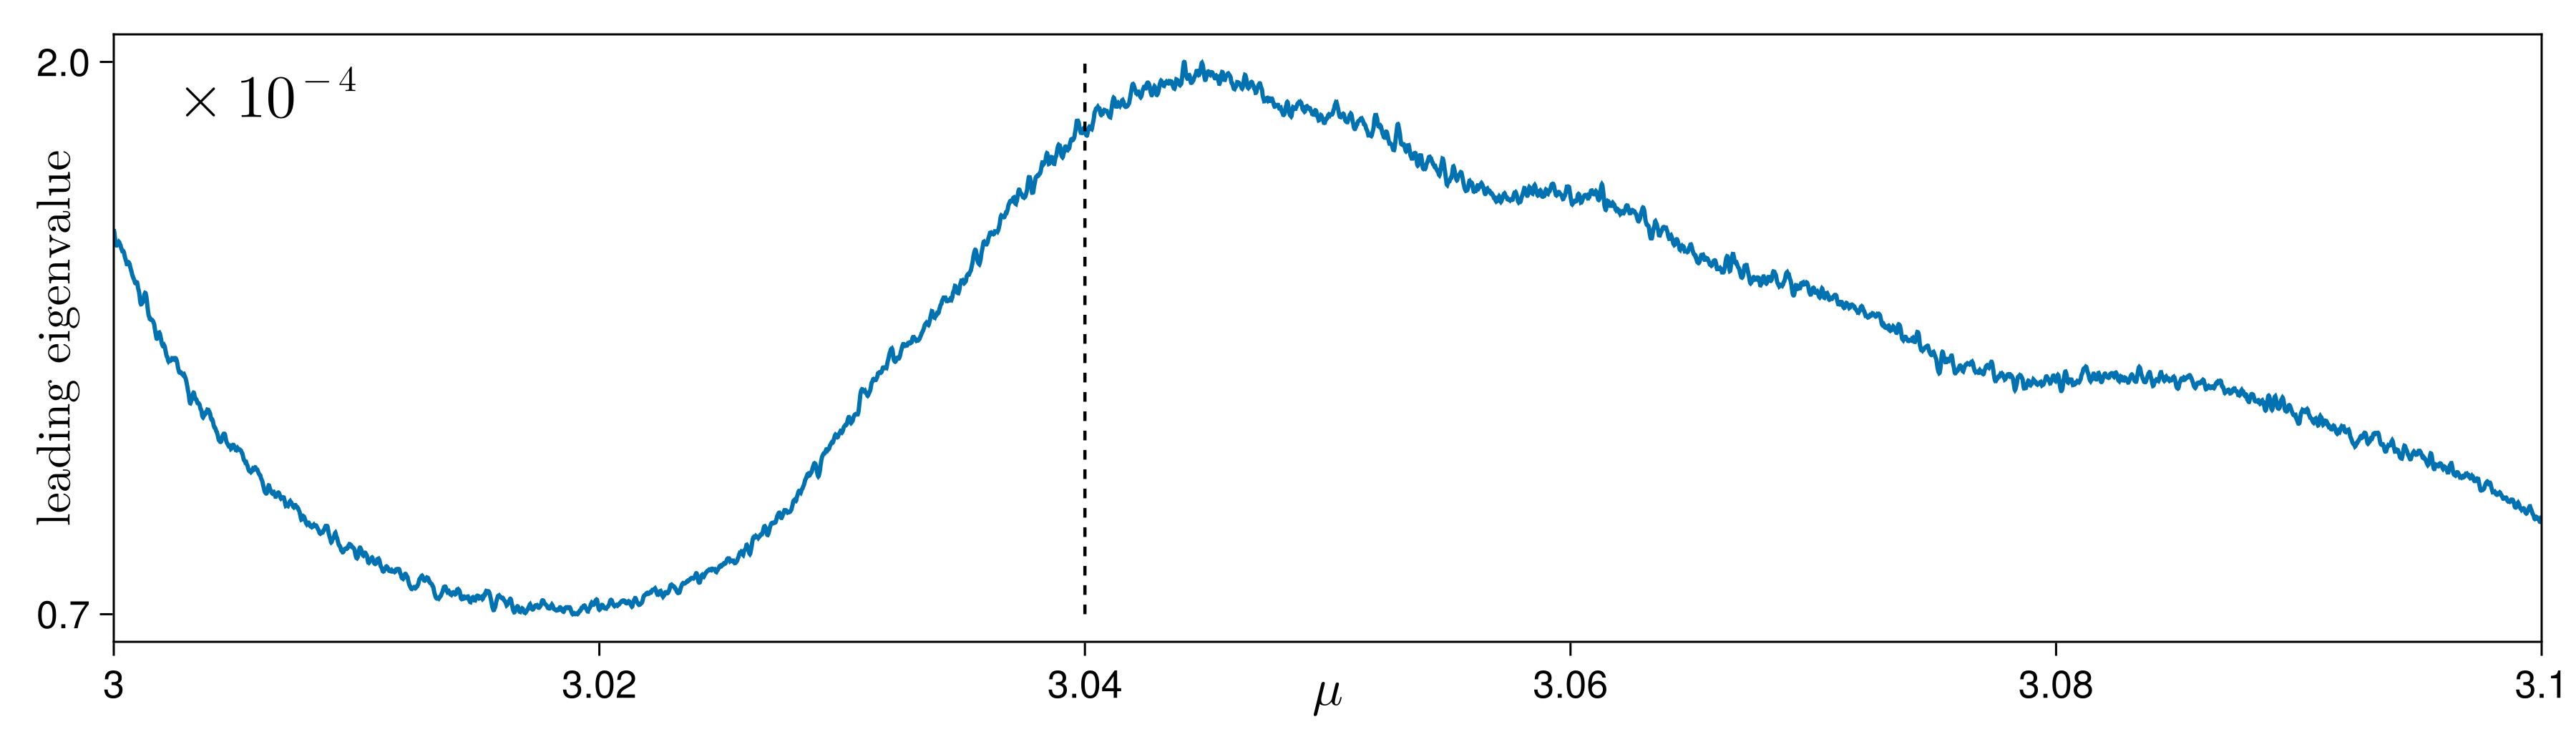
\includegraphics[keepaspectratio, width = \linewidth]{../figures/fig3.8.1.png}
    \end{subfigure}


    \begin{subfigure}[b]{0.11\textwidth}
        \centering 
        
\includegraphics[keepaspectratio, width = \linewidth]{../figures/fig3.8.2.1.png}
    \end{subfigure}
    \hfill
    \begin{subfigure}[b]{0.11\textwidth}
        \centering 
        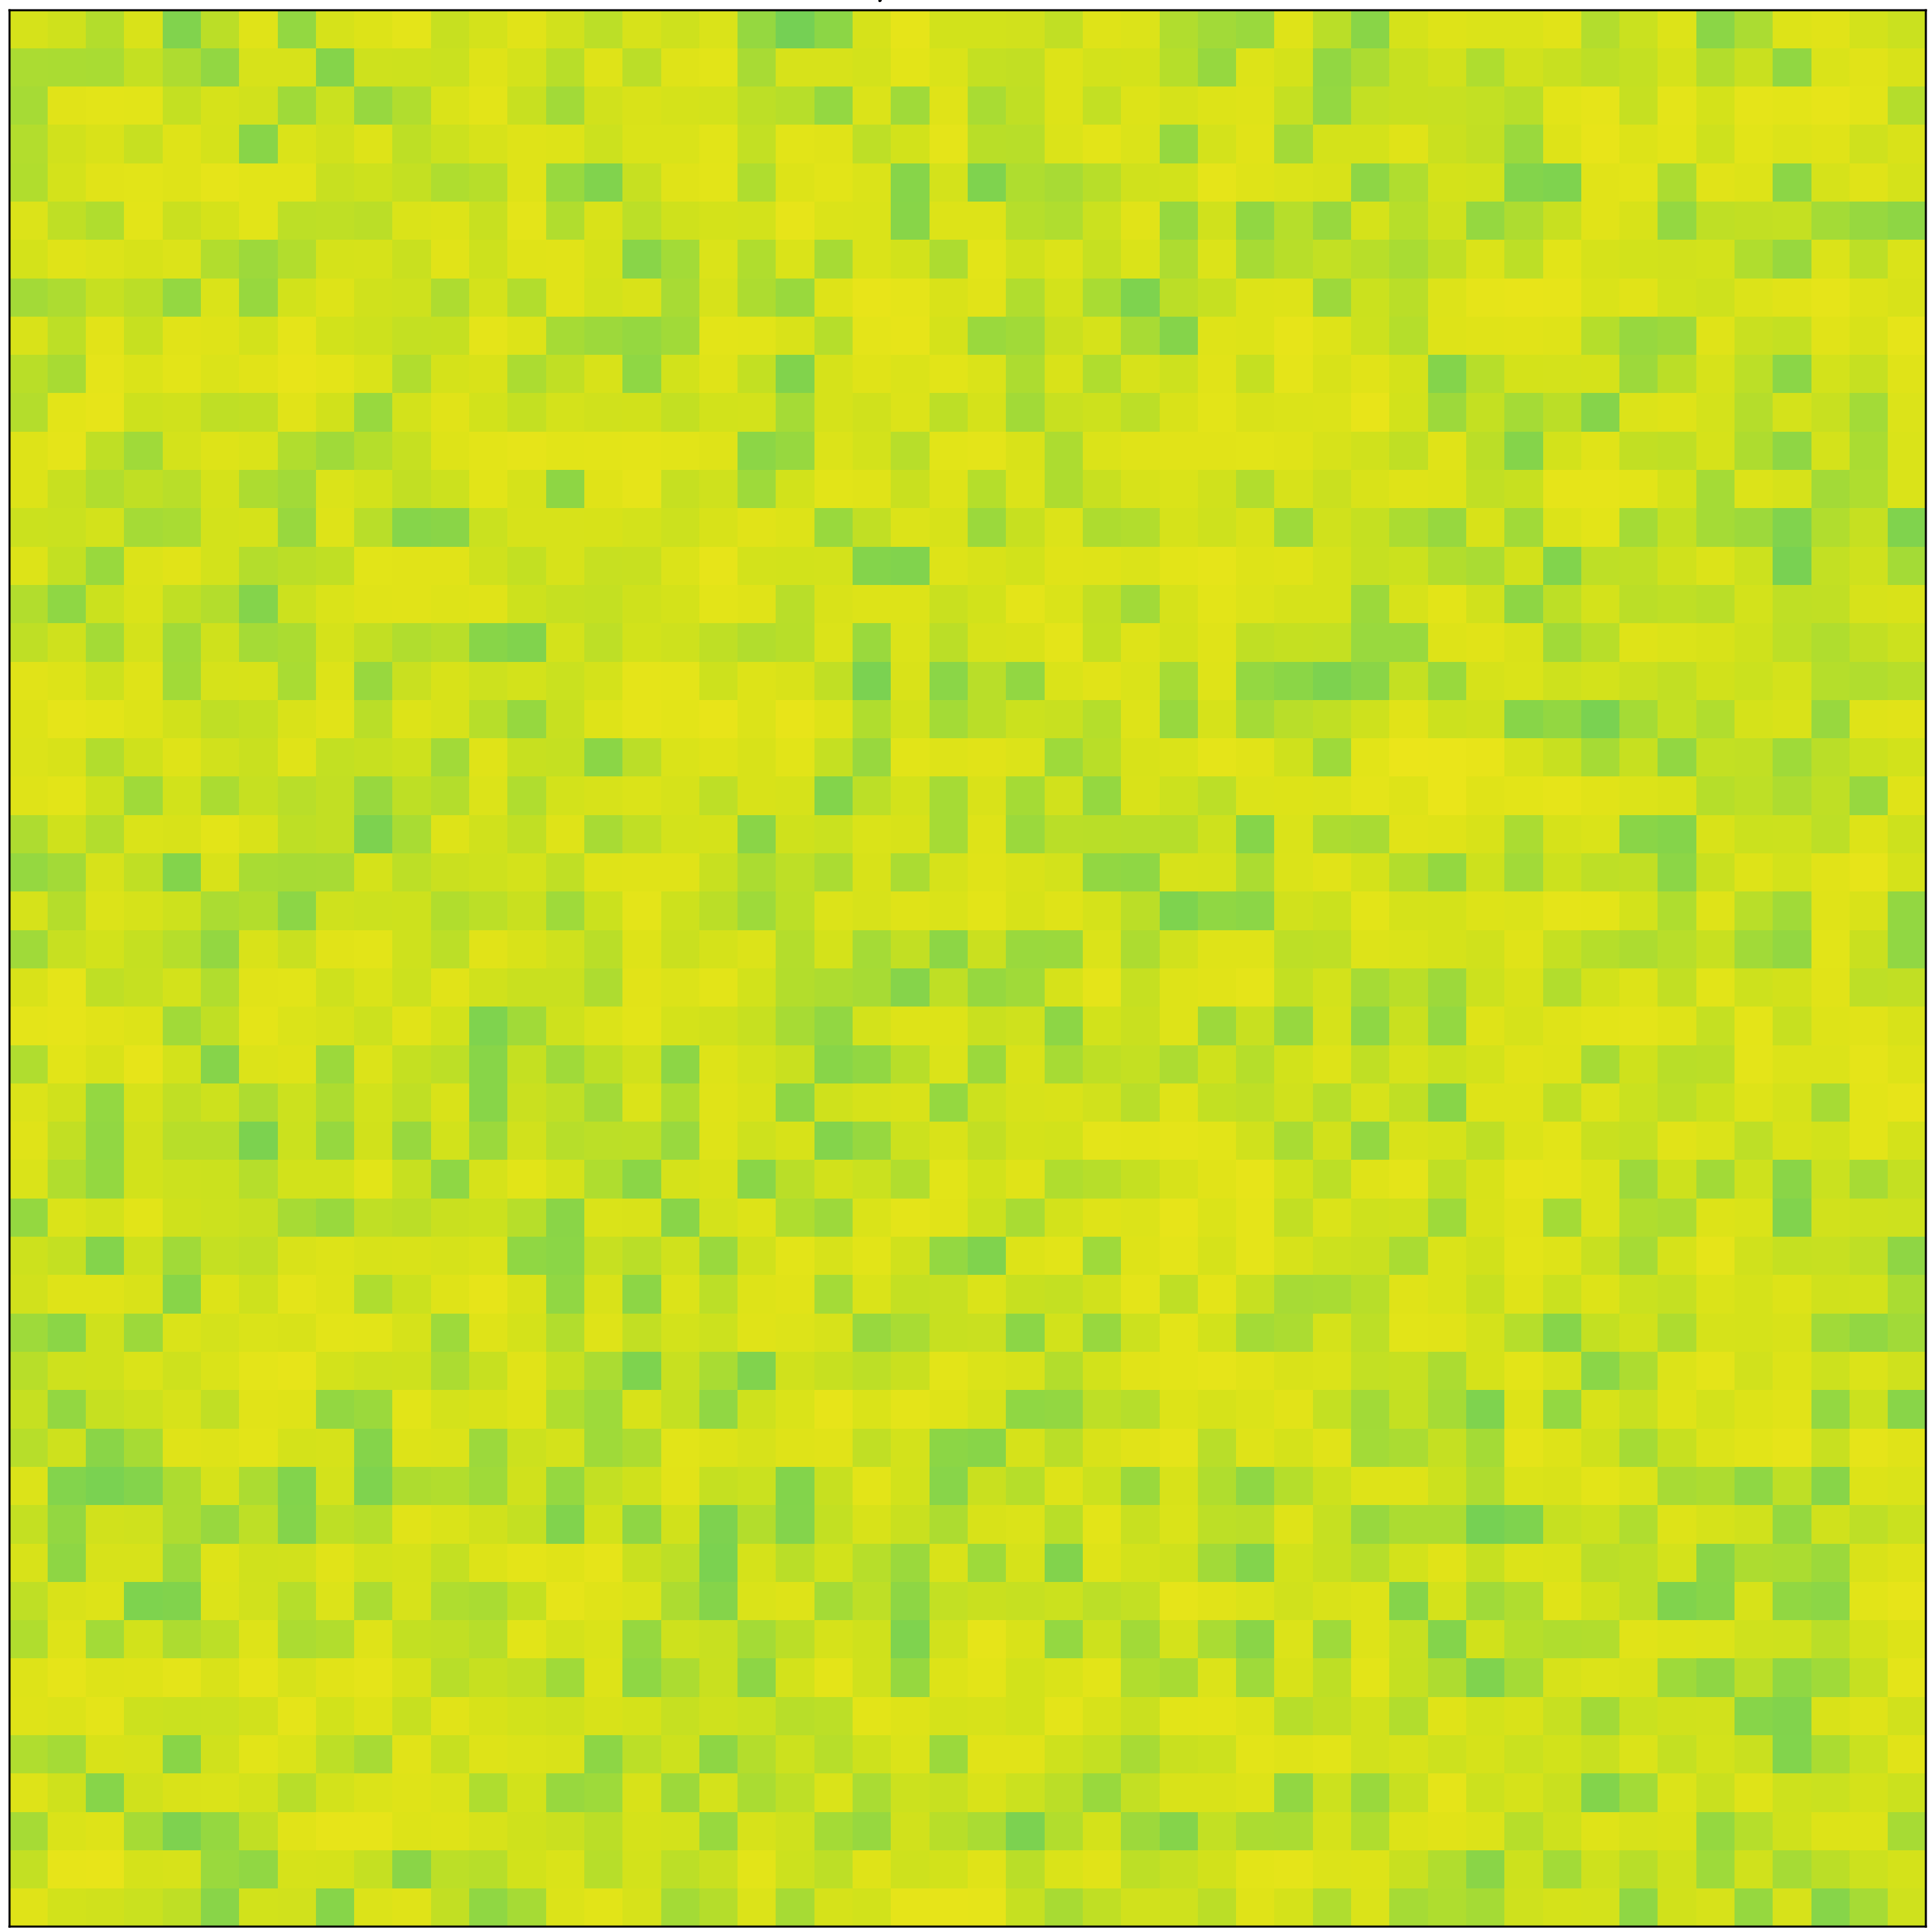
\includegraphics[keepaspectratio, width = \linewidth]{../figures/fig3.8.2.2.png}
    \end{subfigure}
    \hfill
    \begin{subfigure}[b]{0.11\textwidth}
        \centering 
        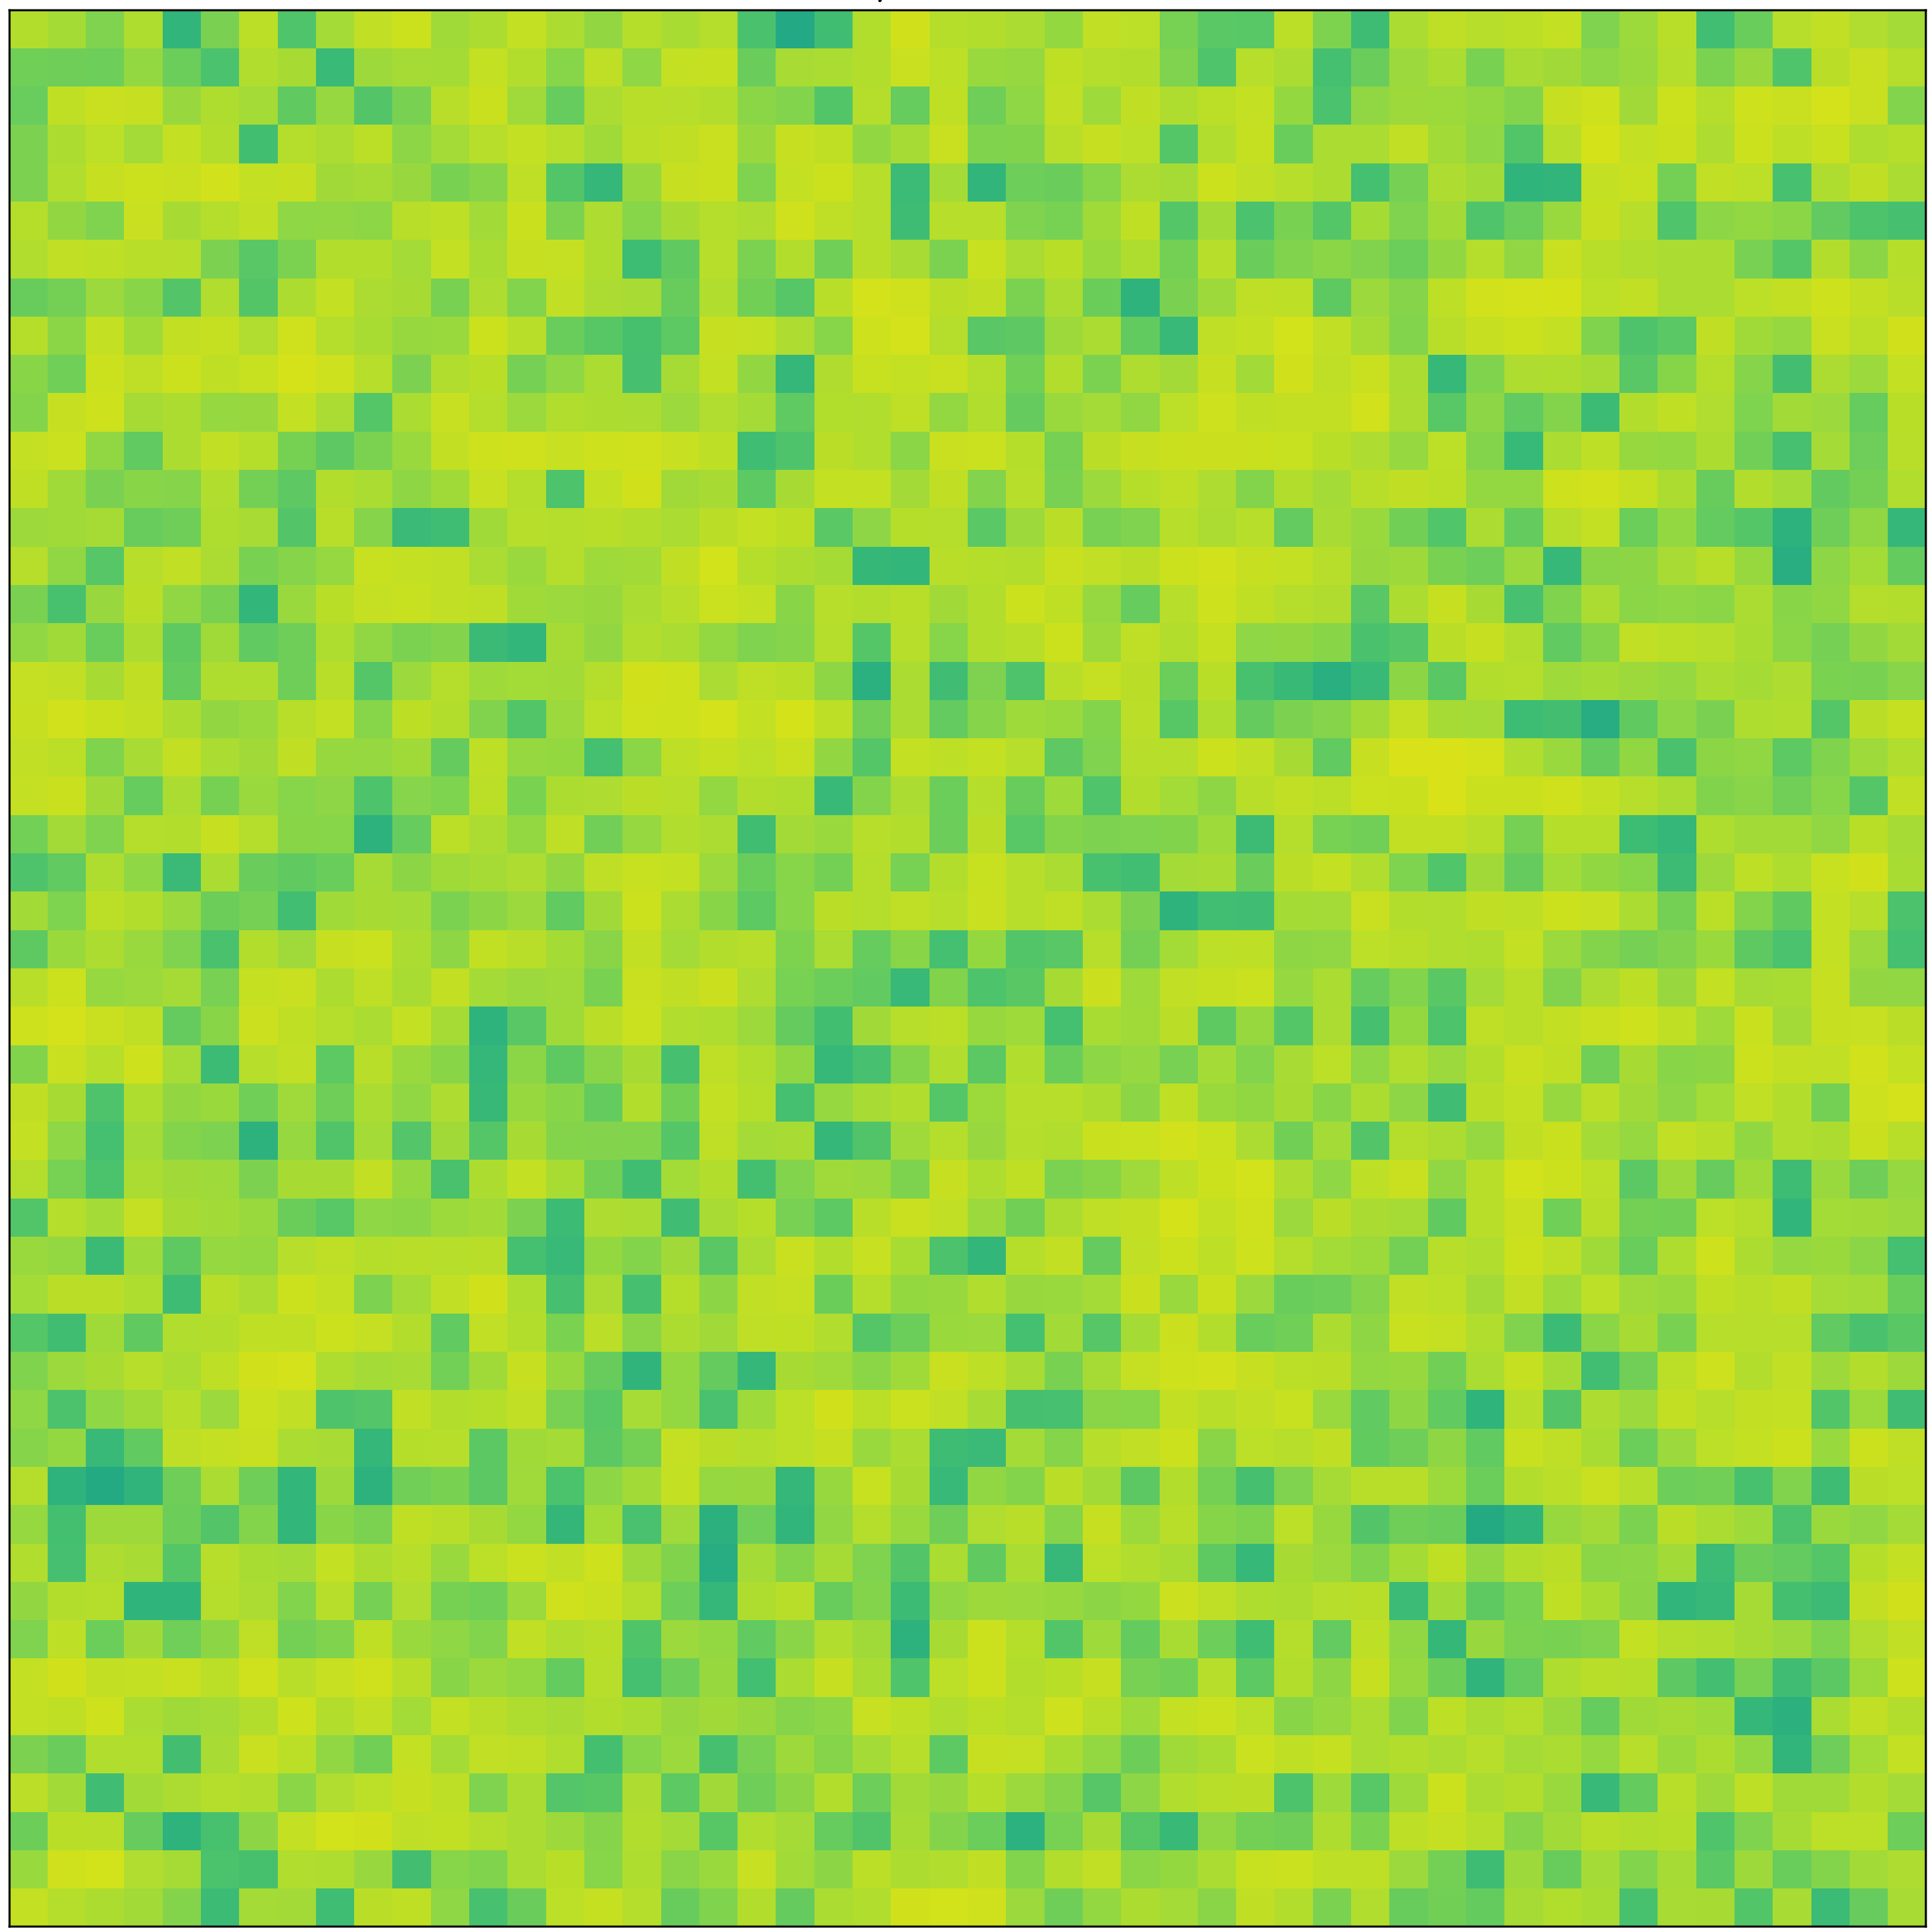
\includegraphics[keepaspectratio, width = \linewidth]{../figures/fig3.8.2.3.png}
    \end{subfigure}
    \hfill
    \begin{subfigure}[b]{0.11\textwidth}
        \centering 
        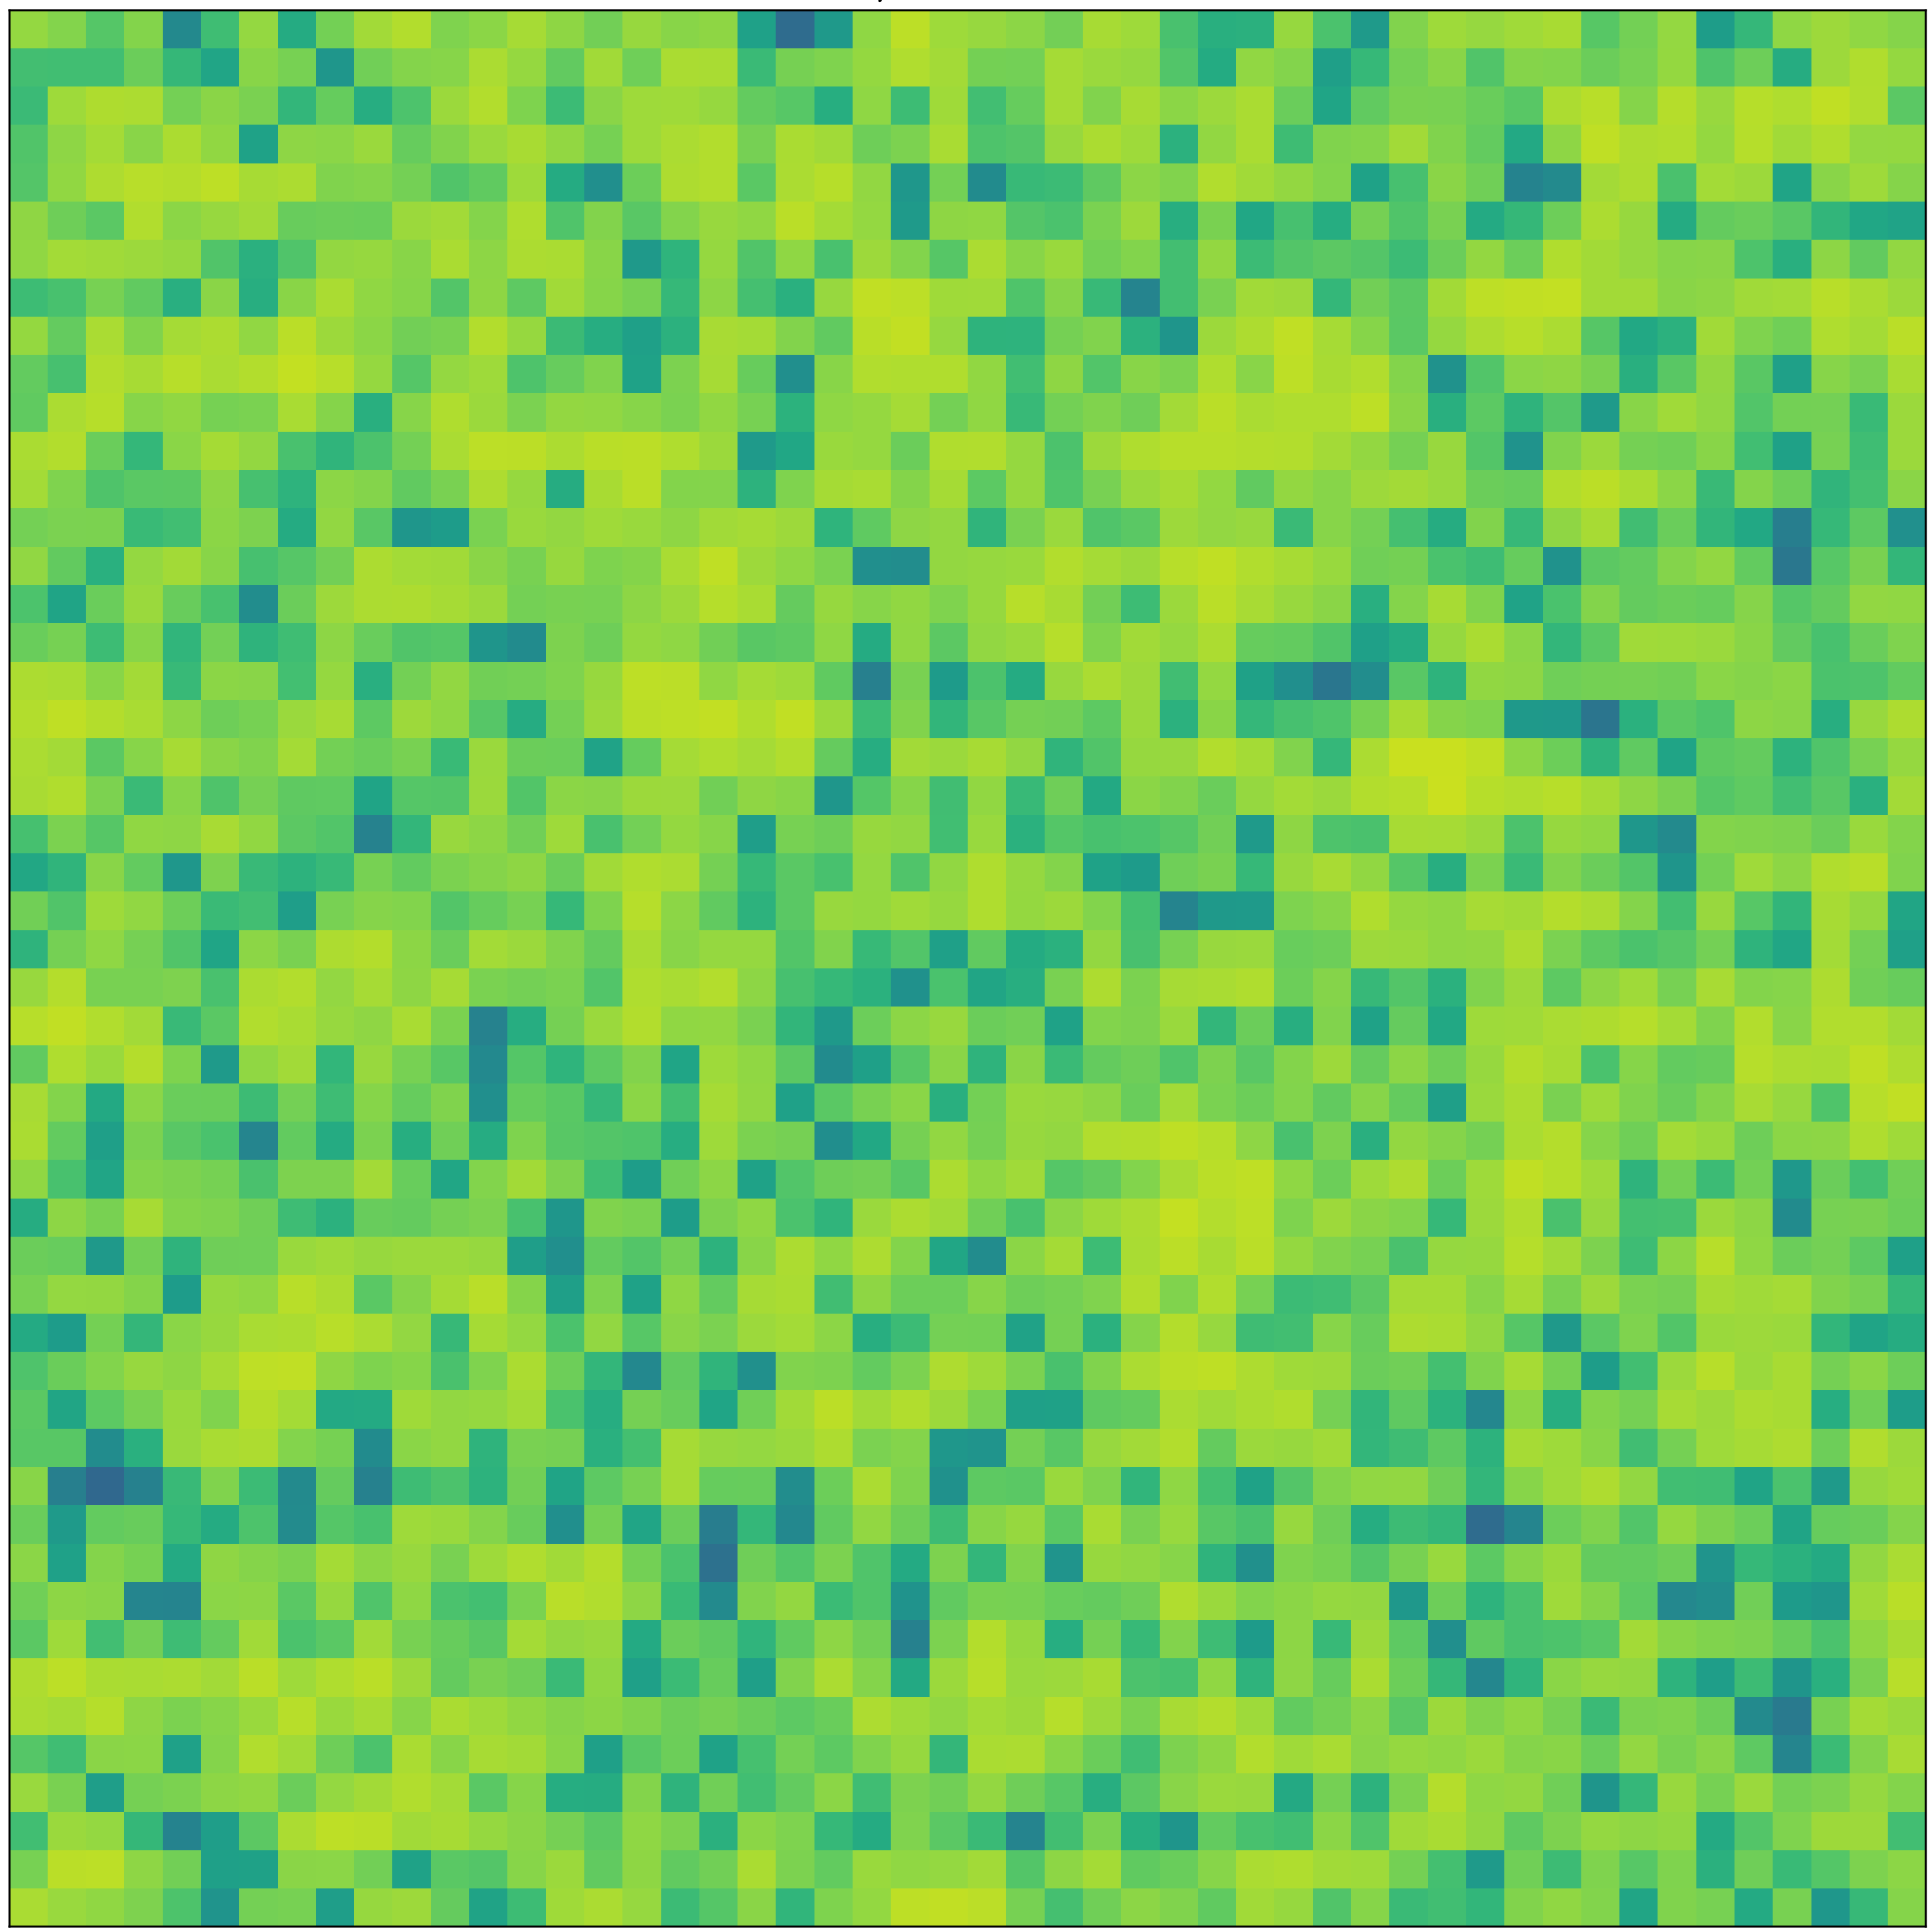
\includegraphics[keepaspectratio, width = \linewidth]{../figures/fig3.8.2.4.png}
    \end{subfigure}
    \hfill
    \begin{subfigure}[b]{0.11\textwidth}
        \centering 
        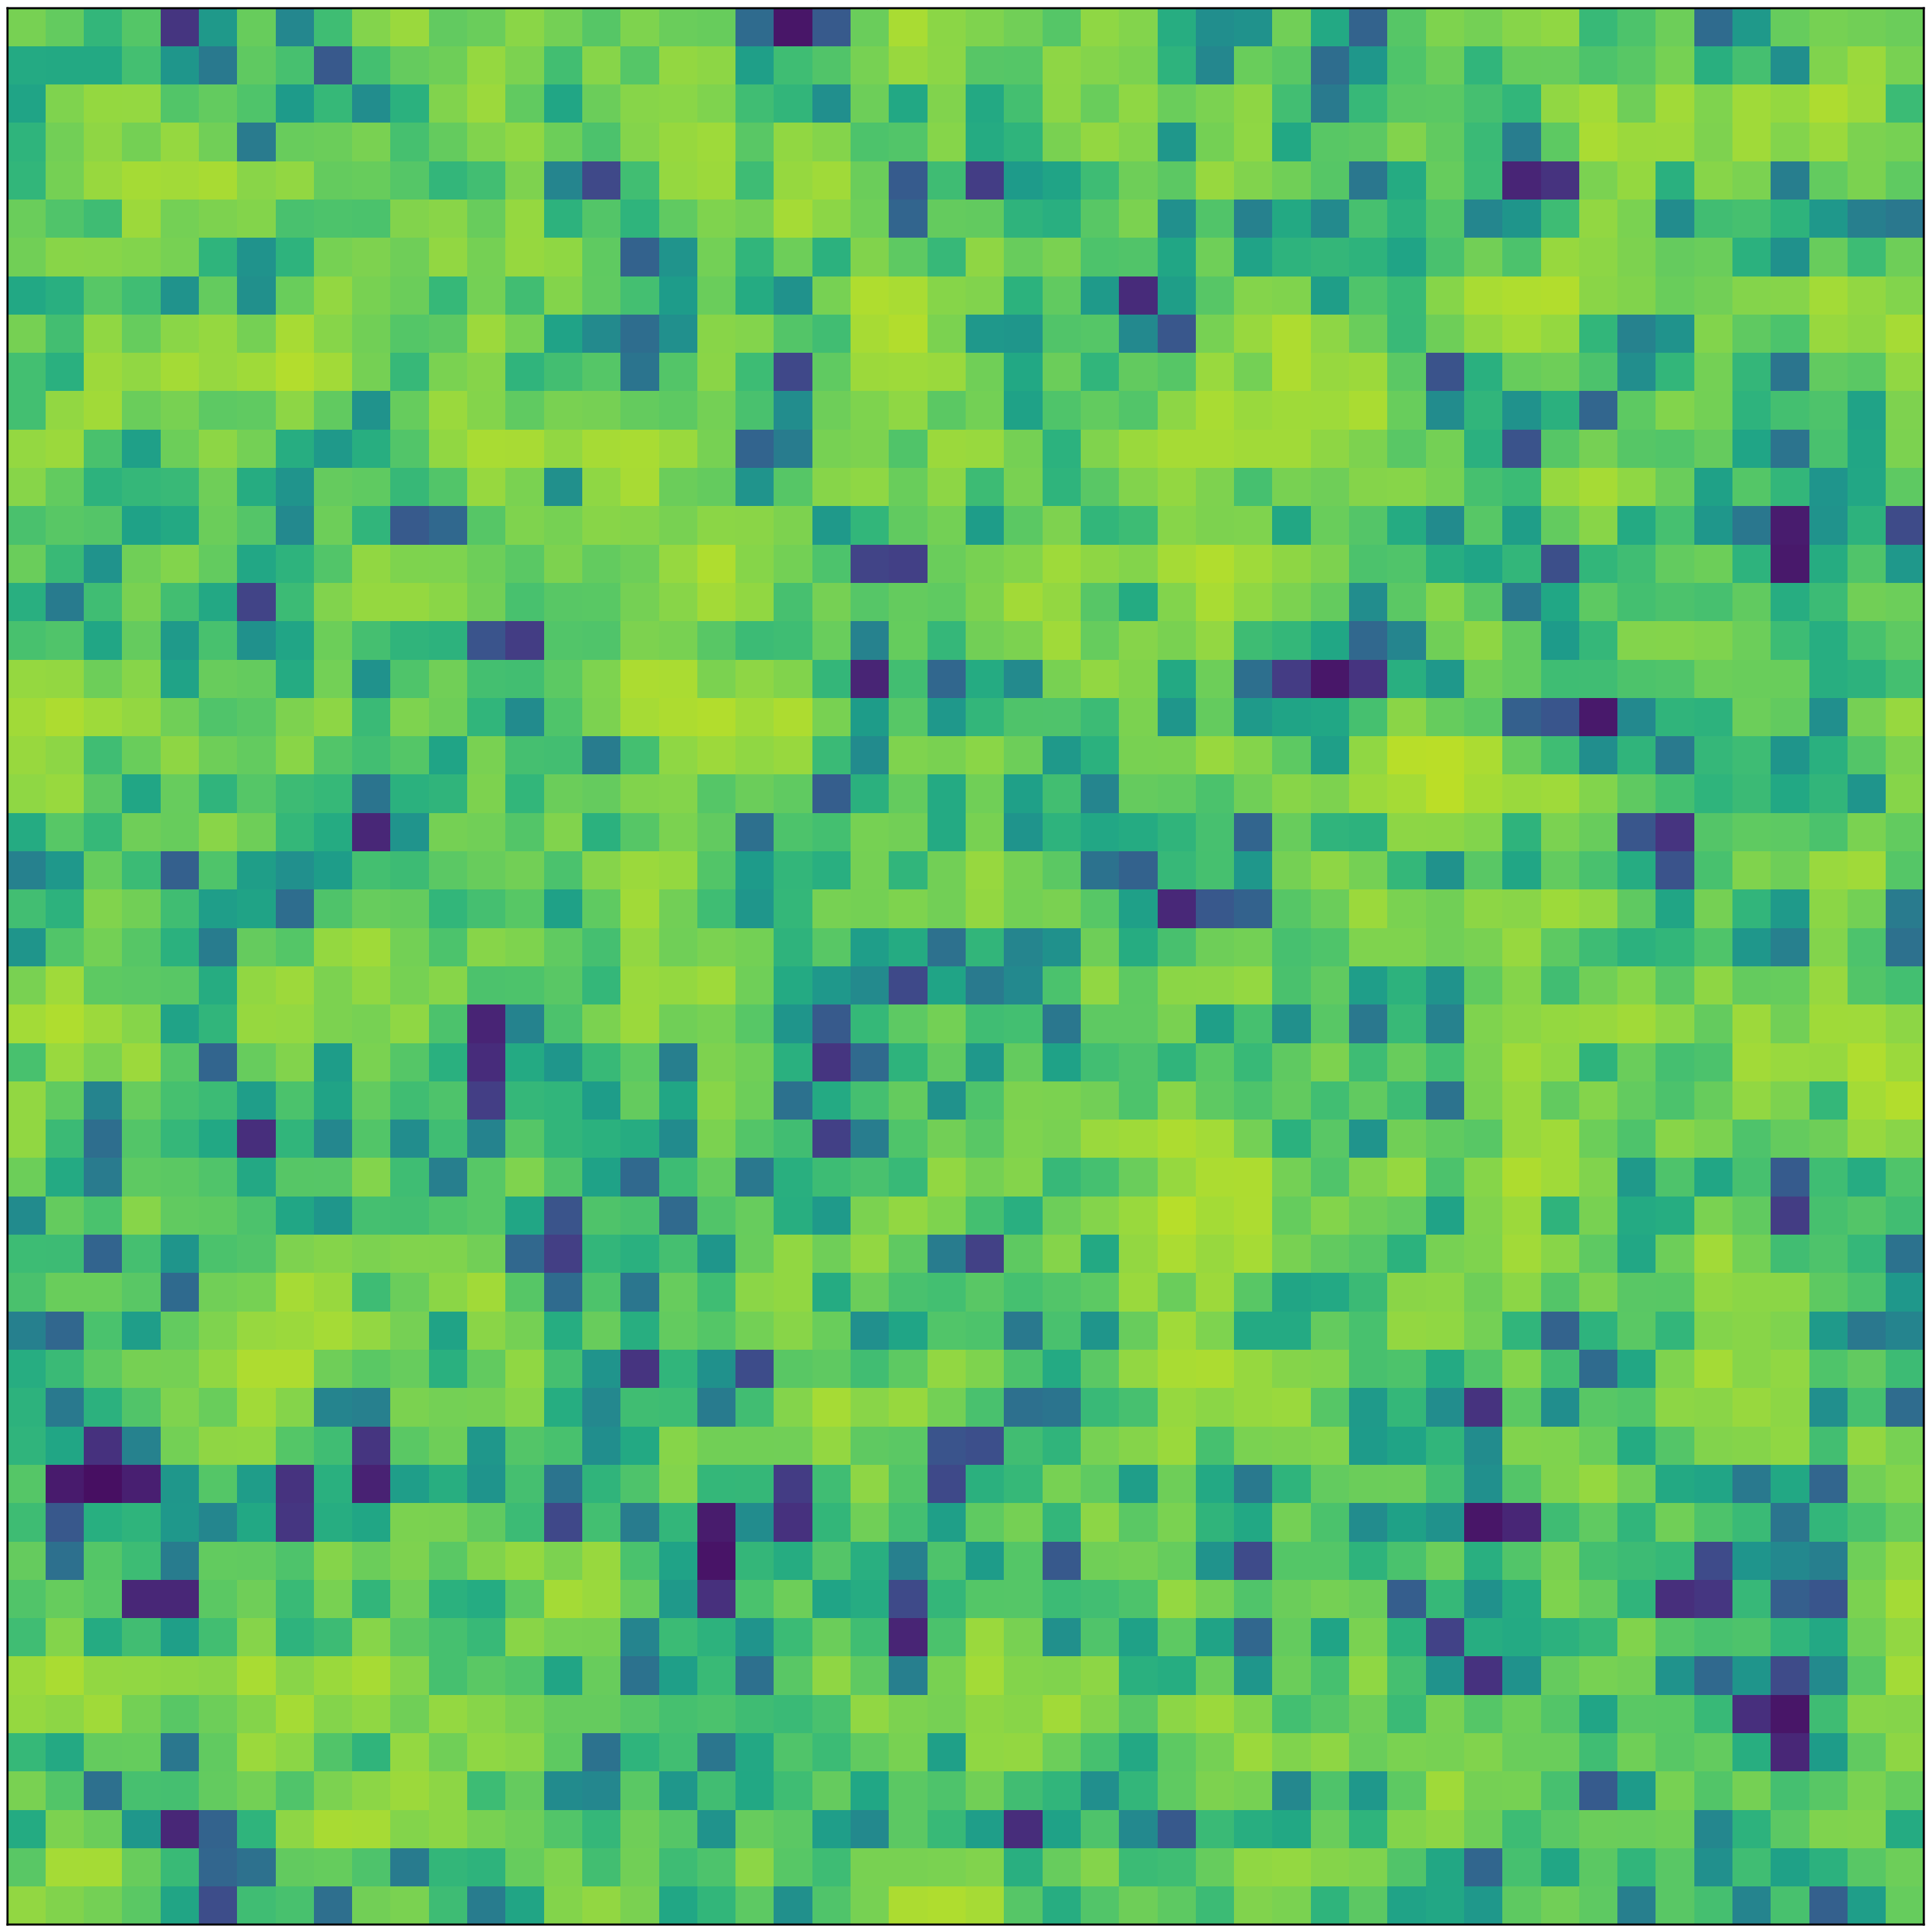
\includegraphics[keepaspectratio, width = \linewidth]{../figures/fig3.8.2.5.png}
    \end{subfigure}
    \hfill
    \begin{subfigure}[b]{0.11\textwidth}
        \centering 
        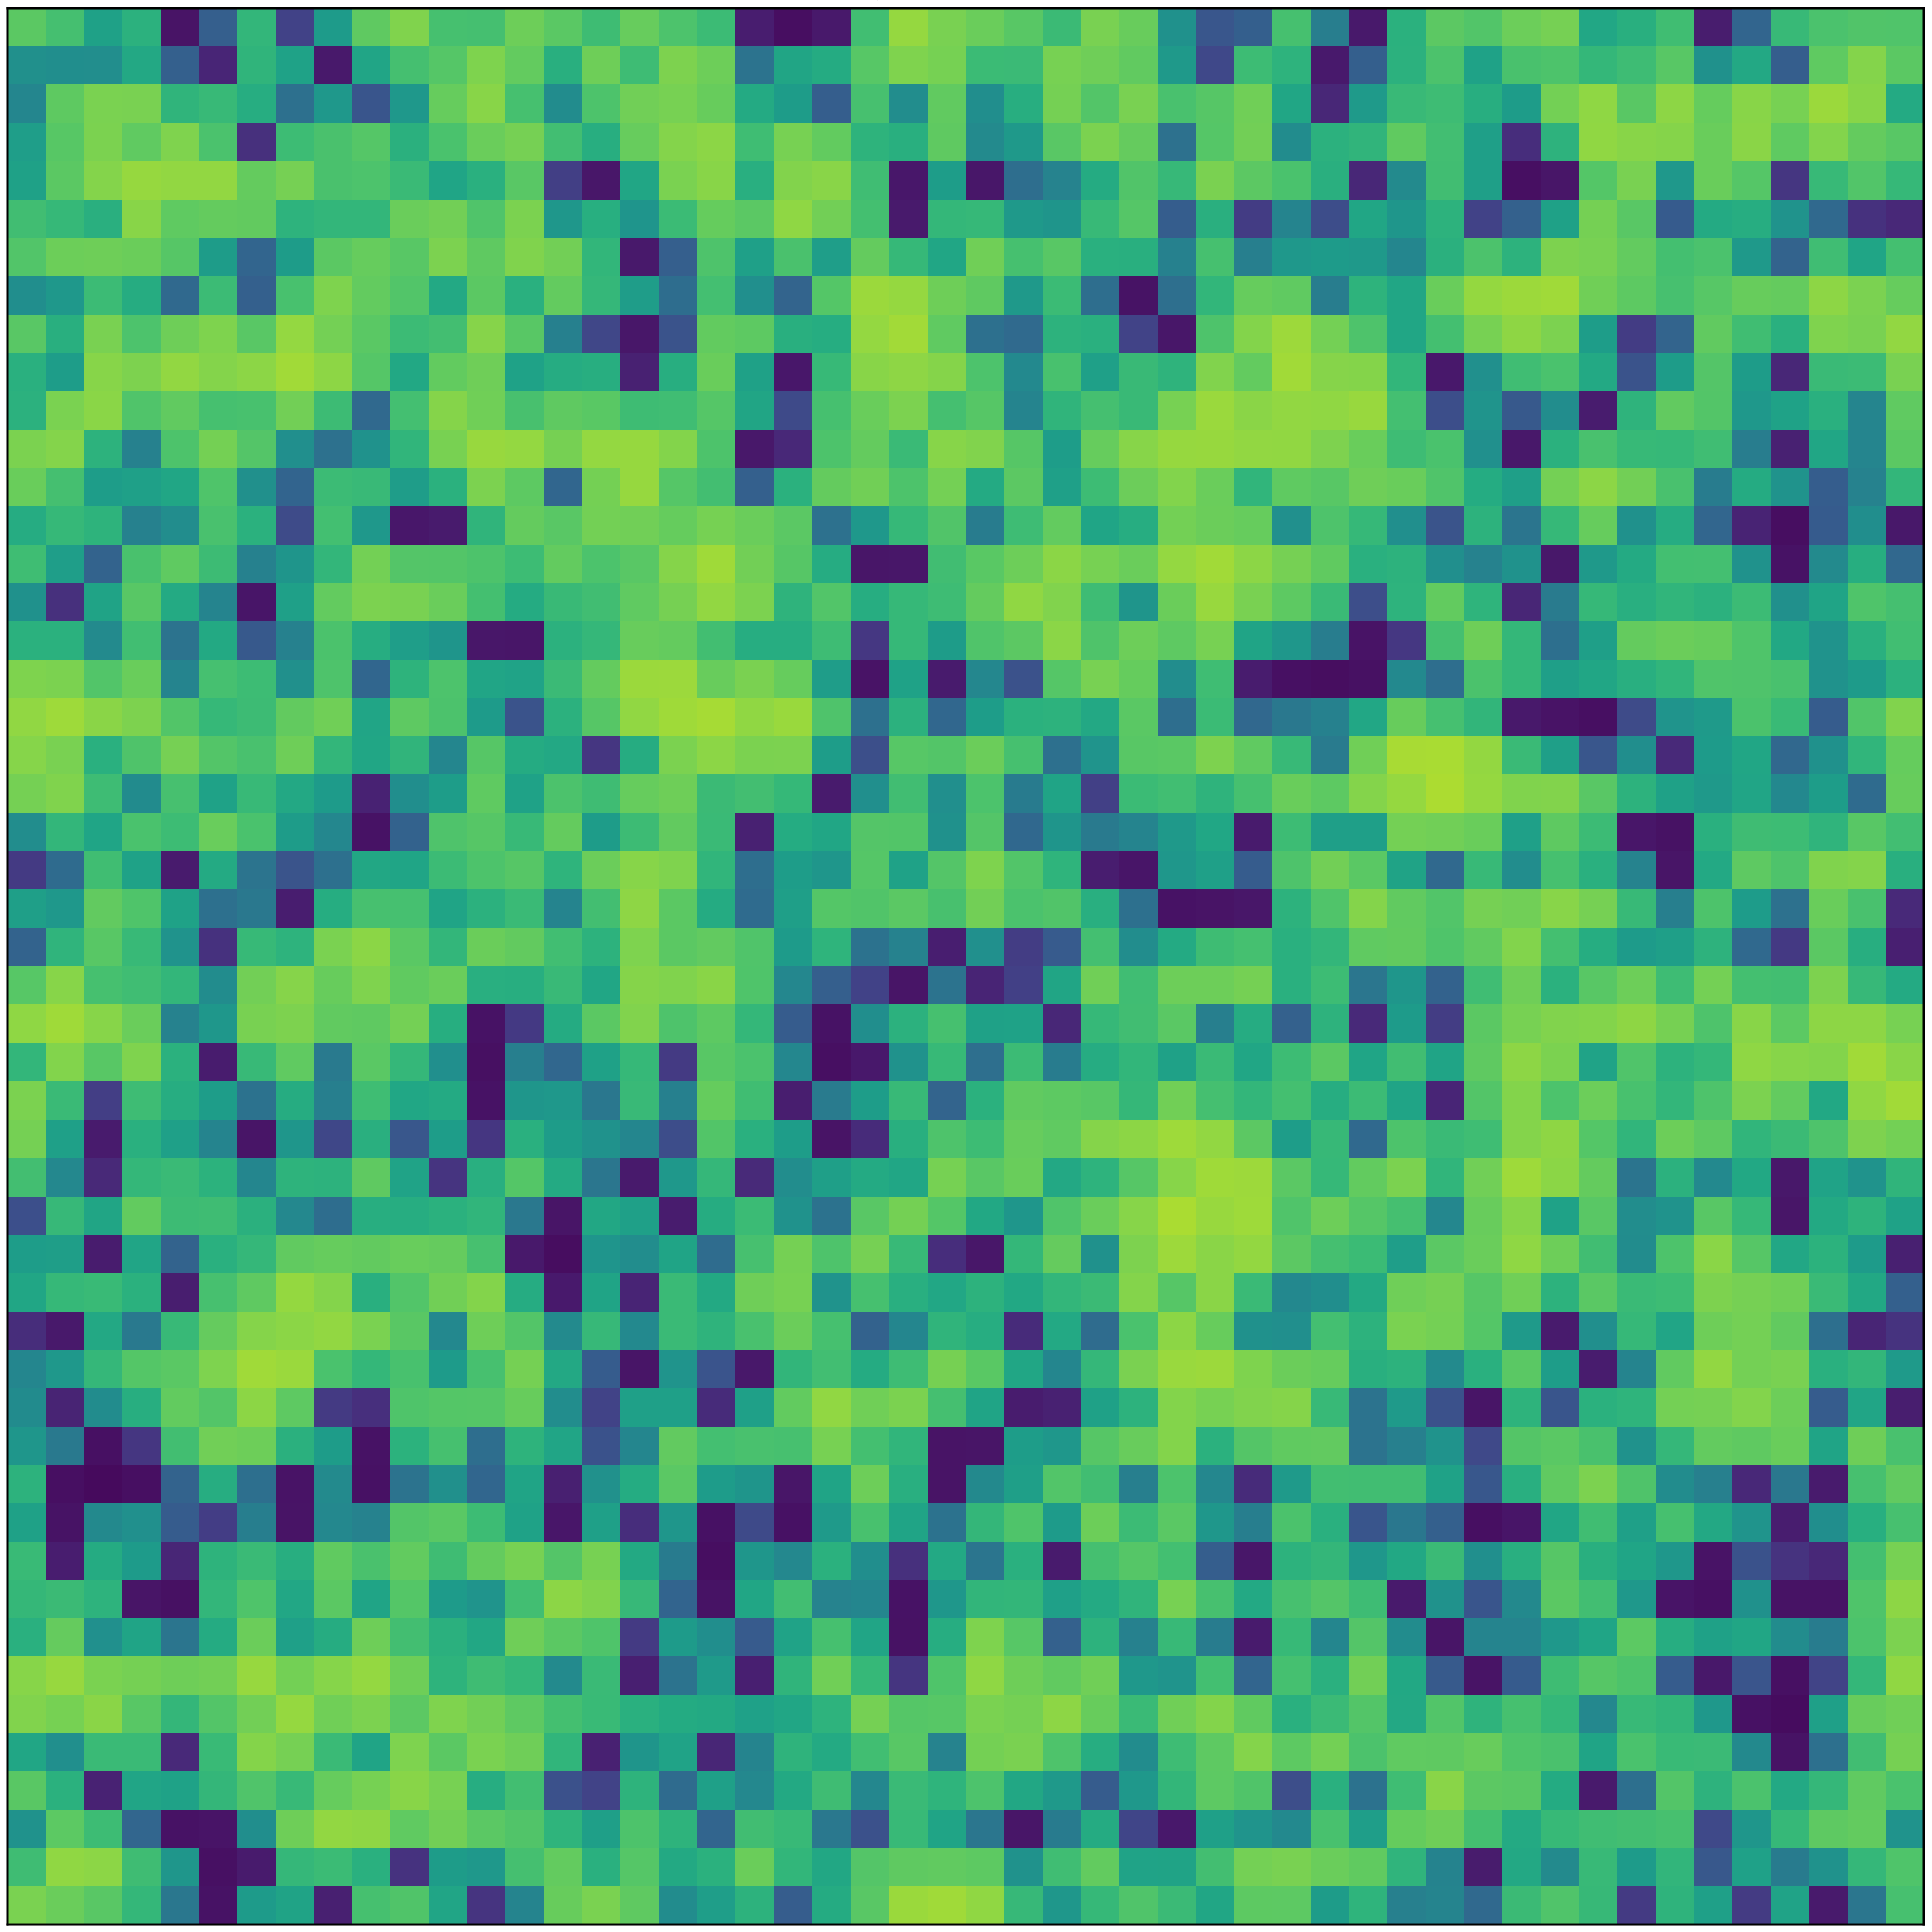
\includegraphics[keepaspectratio, width = \linewidth]{../figures/fig3.8.2.6.png}
    \end{subfigure}
    \hfill
    \begin{subfigure}[b]{0.11\textwidth}
        \centering 
        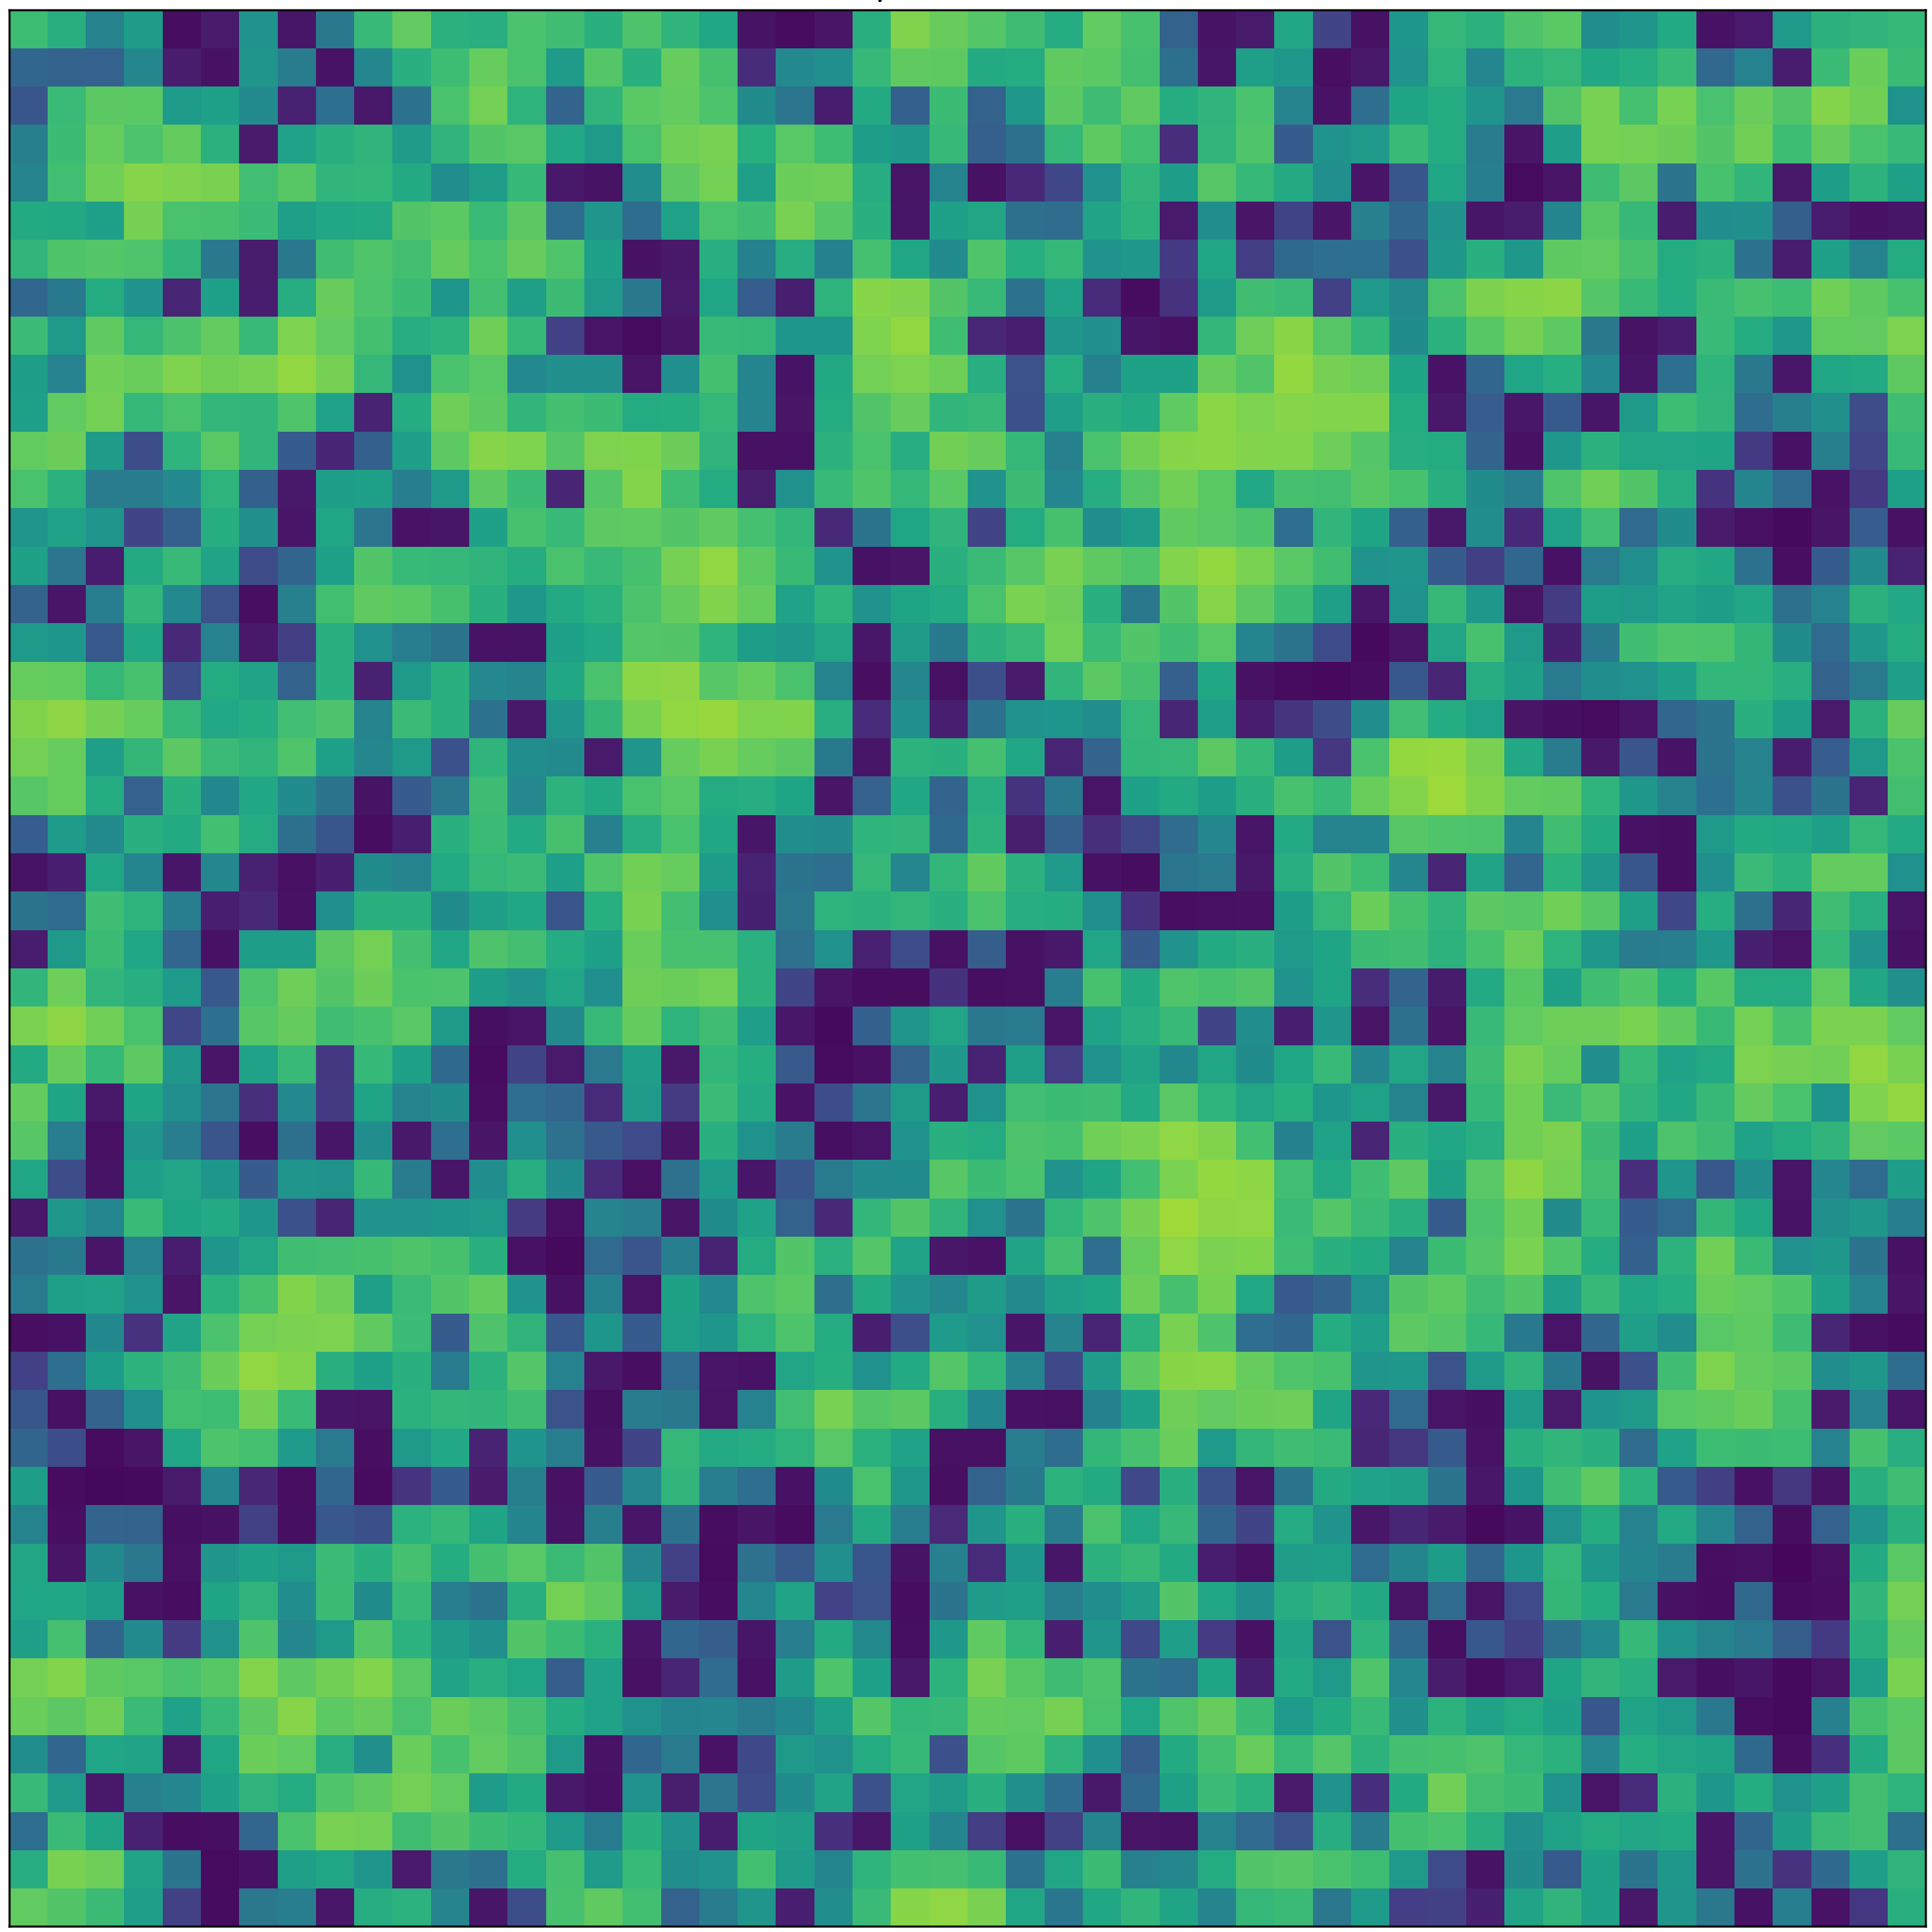
\includegraphics[keepaspectratio, width = \linewidth]{../figures/fig3.8.2.7.png}
    \end{subfigure}
    \hfill
    \begin{subfigure}[b]{0.11\textwidth}
        \centering 
        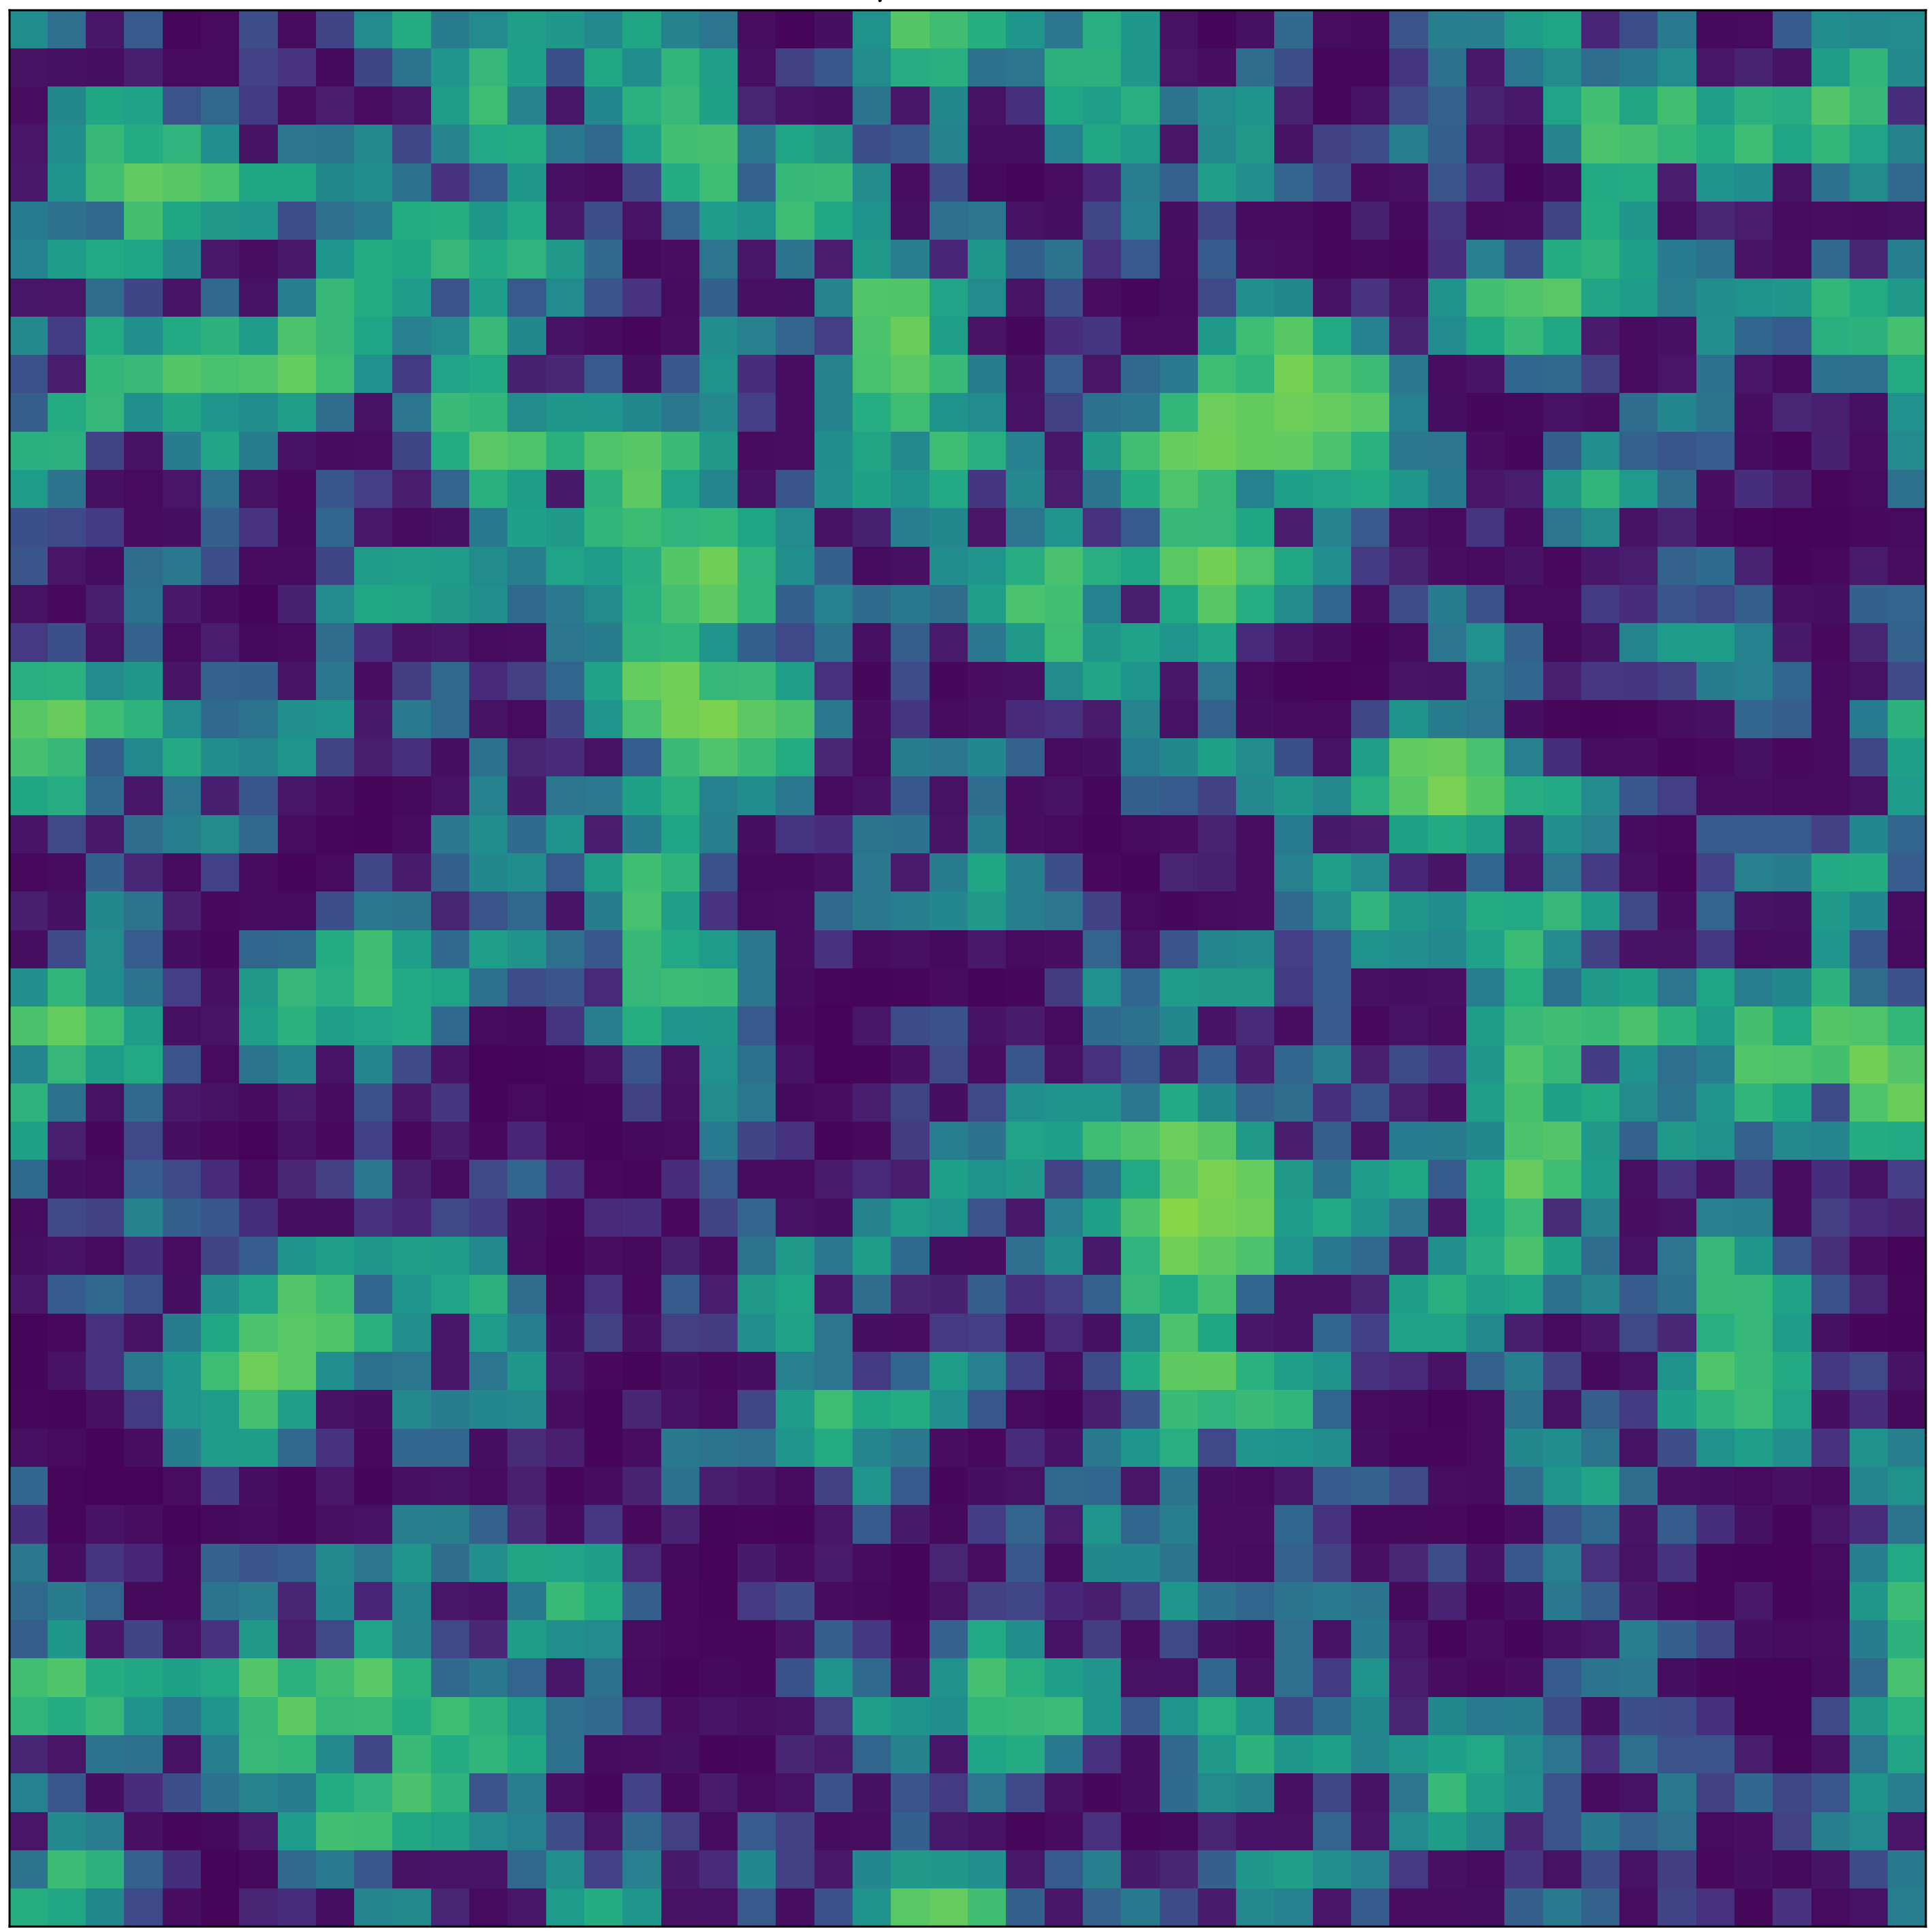
\includegraphics[keepaspectratio, width = \linewidth]{../figures/fig3.8.2.8.png}
    \end{subfigure}
    \caption{Time evolution of the vegetation turbidity LDS on a square $50\times50$ lattice with slow ($\varepsilon=10^{-2}$), linear ramping of the bifurcation parameter, noise level $\sigma=10^{-3}$ and uniform reaction $R=1$ and diffusion $D=0.2$.
The top pannel shows the timeseries of the leading eigenvalue of the covariance matrix assembled over a window of $W=20$ snapshots. 
The dashed vertical line indicates the visual detection of irregular patterns forming in the solution, shown in the bottom panels at increasing timesteps (left to right).}
    \label{fig3.8}
\end{figure}
The fundamental idea behind this analysis is to bring together the spatial and temporal variation of the observables in a (prebefarbly unique) measure that is capable of capturing, with robustness and mathematical interpretability the onset of pattern-formation in spatially extended dynamical systems.
This concept is further investigated in \cite{Donovan22} where the dynamic mode decomposition (DMD) of the Koopman operator linearising the evolution of the reaction-diffusion LDS is employed.
Suppose $\boldsymbol{\mathcal{X}}$ is collecting snapshots from timestep $t_{w}$ to $t_{w+W}$ while in $\boldsymbol{\mathcal{\newprime{X}}}$ we store the snapshots one stride of the sliding window away i.e. capturing the snapshots from $t_{w+S}$ to $t_{(w+S)+W}$.
The DMD will provide us with a more direct and efficient way of capturing CSD and Turing instability by way of approximating the linearisation around the steady-state directly as per the following result.
\begin{theorem}[label=thm3.6]{}{}
     Let $A:\boldsymbol{\mathcal{X}}\to \boldsymbol{\mathcal{\newprime{X}}}$ be a linear operator and $\boldsymbol{\mathcal{X}}\approx \boldsymbol{U}\boldsymbol{\Sigma}\boldsymbol{V}^{T}$ be the singular valued decomposition (SVD) of $\boldsymbol{\mathcal{X}}$, then the spectrum of $\boldsymbol{S}:= \boldsymbol{U}^{T}\boldsymbol{\mathcal{\newprime{X}}}\boldsymbol{V}\boldsymbol{\Sigma}^{-1}$ is the best approximation of the spectrum of A ($\sigma(A)$) and its eigenvectors are also optimally approximated by those of $\boldsymbol{S}$ multiplied from the left by $\boldsymbol{U}$.
\end{theorem}
\begin{proof}
        Here $\boldsymbol{\mathcal{X}}$ will represent a matrix of snapshots of the solution at different timesteps over the square $N-$dimensional lattice (i.e. $N:=n^{2}$) collected across a sliding window of fixed width $W$.
     Since $\boldsymbol{\mathcal{X}}\in \mathbb{R}^{N\times W}$ then the SVD will give us the left and right singular vectors in $\boldsymbol{U}$, $\boldsymbol{V}\in \mathbb{R}^{N\times W}$ respectively while the singular values will be stored along the (main) diagonal of $\boldsymbol{\Sigma}\in \mathbb{R}^{W\times W}$ (which is not the covariance matrix as in the previous case).
     From straightforward algebraic manipulation we get
     \begin{equation*}
          A = \boldsymbol{\mathcal{\newprime{X}}}\boldsymbol{\mathcal{X}}^{-1}\approx \boldsymbol{\mathcal{\newprime{X}}}(\boldsymbol{U}\boldsymbol{\Sigma}\boldsymbol{V}^{T})^{-1}=\boldsymbol{\mathcal{\newprime{X}}}\boldsymbol{V}^{-T}\boldsymbol{\Sigma}^{-1}\boldsymbol{U}^{-1} = \boldsymbol{\mathcal{\newprime{X}}}\boldsymbol{V}\boldsymbol{\Sigma}^{-1}\boldsymbol{U}^{T}\;\Rightarrow\;\boldsymbol{U}^{-1}A \boldsymbol{U}\approx \boldsymbol{U}^{T}\boldsymbol{\mathcal{\newprime{X}}}\boldsymbol{V}\boldsymbol{\Sigma}^{-1}=:\boldsymbol{S}\,,
     \end{equation*}
     where we used the fact that both $\boldsymbol{U}$ and $\boldsymbol{V}$ are orthogonal. The eigendecomposition of $\boldsymbol{S}$ will then give
    \begin{equation*}
         \boldsymbol{U}^{-1}A \boldsymbol{U}\approx \boldsymbol{S}=\boldsymbol{Q}\boldsymbol{\Lambda}\boldsymbol{Q}^{-1}\;\Rightarrow\;A \approx (\boldsymbol{U}\boldsymbol{Q})\boldsymbol{\Lambda}(\boldsymbol{U}\boldsymbol{Q})^{-1}\,.
    \end{equation*}
\end{proof}
As an illustrative example of how the leading eigenvalue of the DMD can provide a prognostic of pattern-formation events here we consider the LDS formulation of a lung ventilation model introduced in \cite{Donovan15}. Again from \eqref{eq3.19} we write
\begin{align}
             \phi(u_{\ell}, u_{\ell\pm1},u_{\ell\pm n};\mu) =&\, \sigma(-r_{\ell})\,, \nonumber \\
            \psi(u_{\ell};\mu) =&\,-u_{\ell} \,,\nonumber
\end{align}
where $\sigma(\theta)=\frac{1}{1+e^{-\theta}}$ is the sigmoid function and 
$$r_{\ell}:=-P_{b}(t)+\mu \frac{k}{u_{\ell}}+P_{b}A(u_{\ell}^{4}+u_{\ell+1}^{4}+u_{\ell-1}^{4}+u_{\ell+n}^{4}+u_{\ell-n}^{4})(1 - 1 - u_{\ell}+ \frac{3}{2}(1-u_{\ell})^{2})\,,$$
with $P_{b}(t):=\frac{P_{b}(0)N}{\sum_{\ell=1}^{N}u_{\ell}^{4}}$. Notice that this last term enforces global-coupling of the lattice sites alongside the traditional local, nearest-neighbour interactions of the discrete diffusion operator.
Finally the remaining homogeneous constants are set to $k=14.1$, $A=0.63$, $P_{i}=0.96$, $P_{b}(0)=7.25$.
In Figure \ref{fig3.10} below we report the detection of the proposed spatio-temporal EWS for this model.
\begin{figure}[H]
    \centering 
    \begin{subfigure}[b]{\textwidth}
        \centering 
        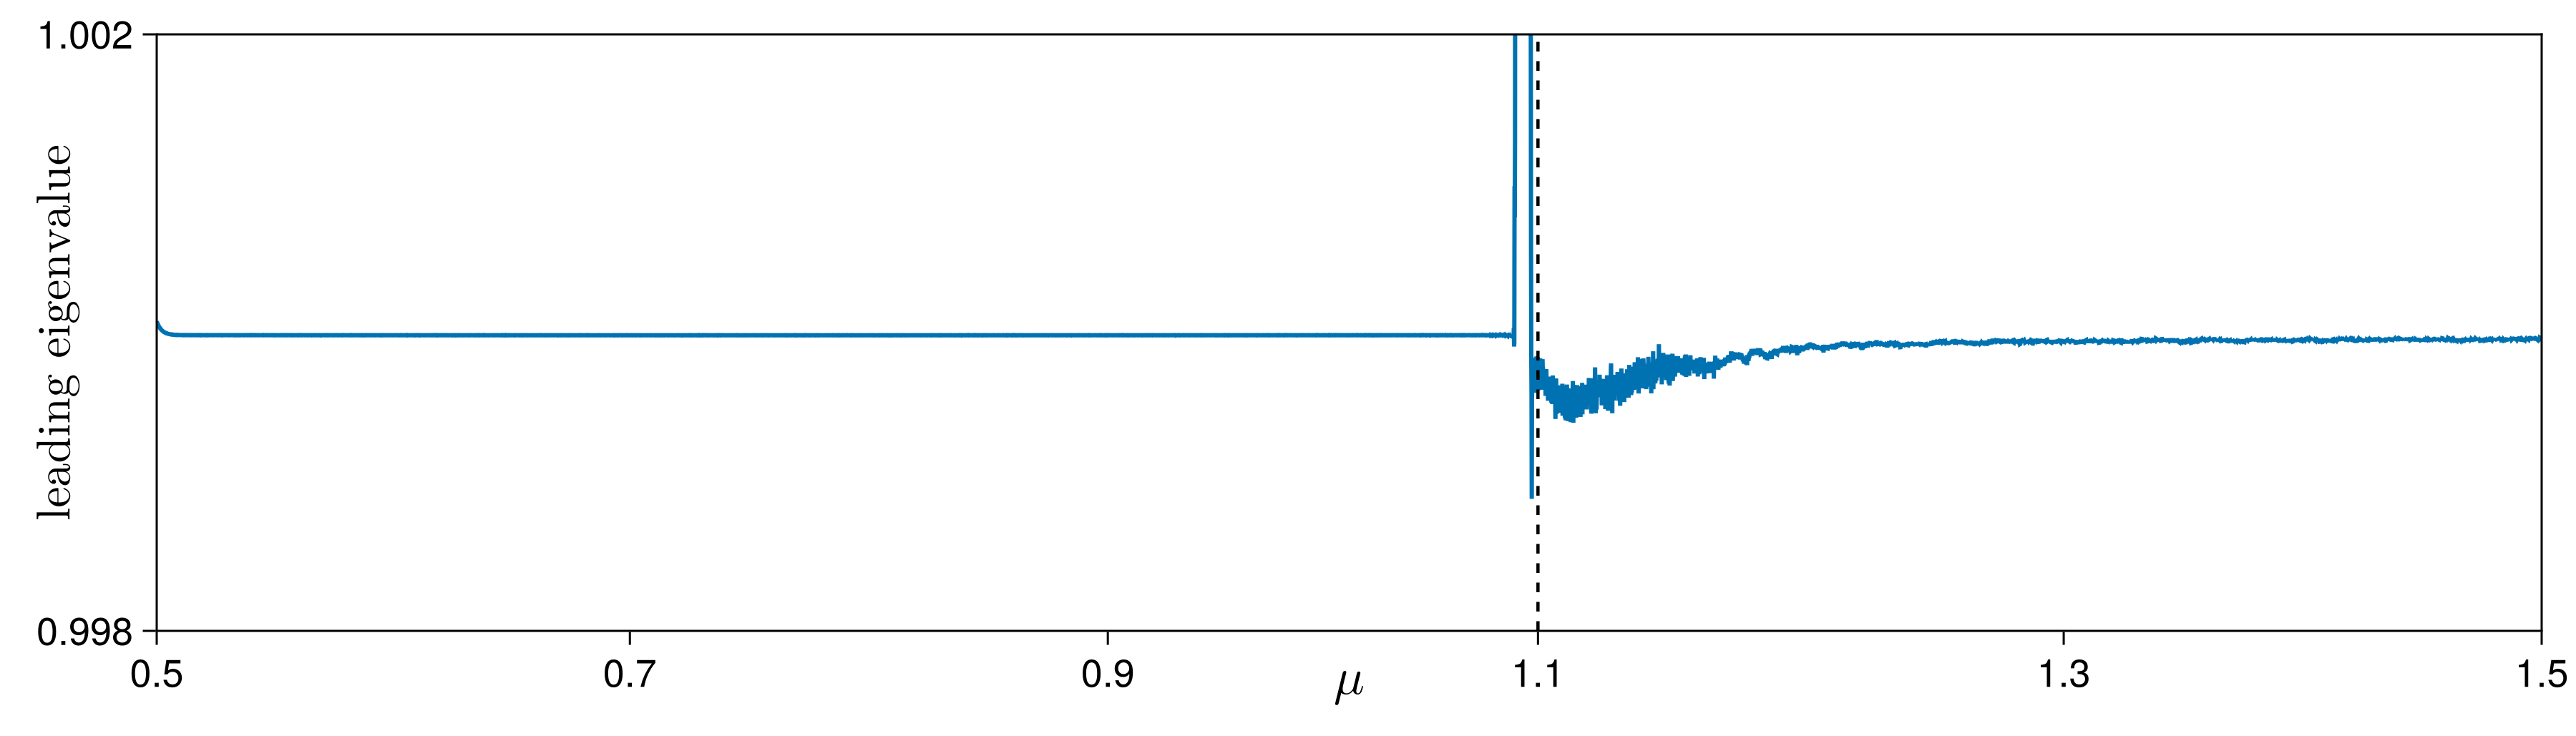
\includegraphics[keepaspectratio, width = \linewidth]{../figures/fig3.9.1.png}
    \end{subfigure}


    \begin{subfigure}[b]{0.11\textwidth}
        \centering 
        
\includegraphics[keepaspectratio, width = \linewidth]{../figures/fig3.9.2.1.png}
    \end{subfigure}
    \hfill
    \begin{subfigure}[b]{0.11\textwidth}
        \centering 
        
\includegraphics[keepaspectratio, width = \linewidth]{../figures/fig3.9.2.2.png}
    \end{subfigure}
    \hfill
    \begin{subfigure}[b]{0.11\textwidth}
        \centering 
        
\includegraphics[keepaspectratio, width = \linewidth]{../figures/fig3.9.2.3.png}
    \end{subfigure}
    \hfill
    \begin{subfigure}[b]{0.11\textwidth}
        \centering 
        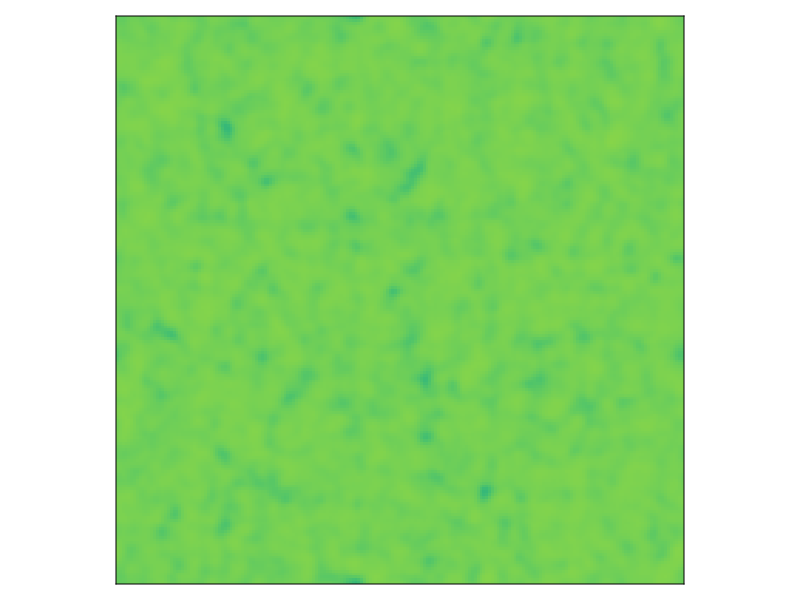
\includegraphics[keepaspectratio, width = \linewidth]{../figures/fig3.9.2.4.png}
    \end{subfigure}
    \hfill
    \begin{subfigure}[b]{0.11\textwidth}
        \centering 
        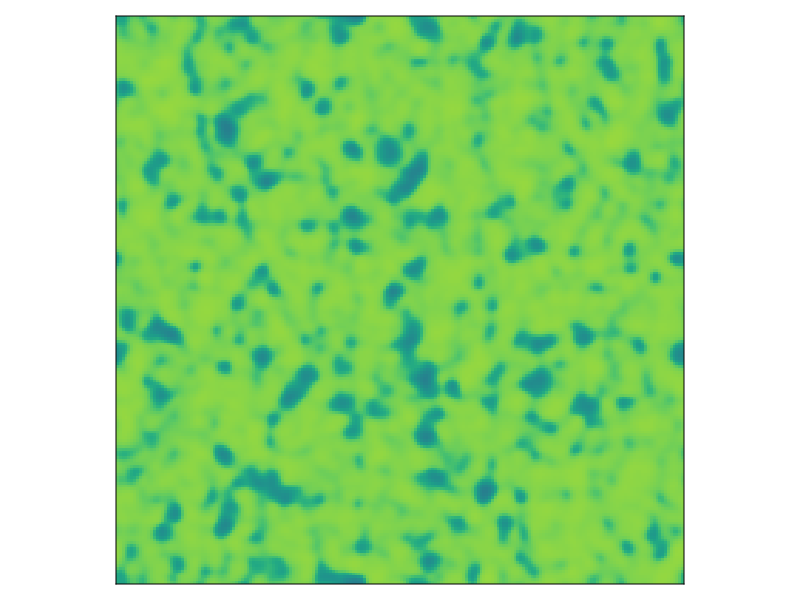
\includegraphics[keepaspectratio, width = \linewidth]{../figures/fig3.9.2.5.png}
    \end{subfigure}
    \hfill
    \begin{subfigure}[b]{0.11\textwidth}
        \centering 
        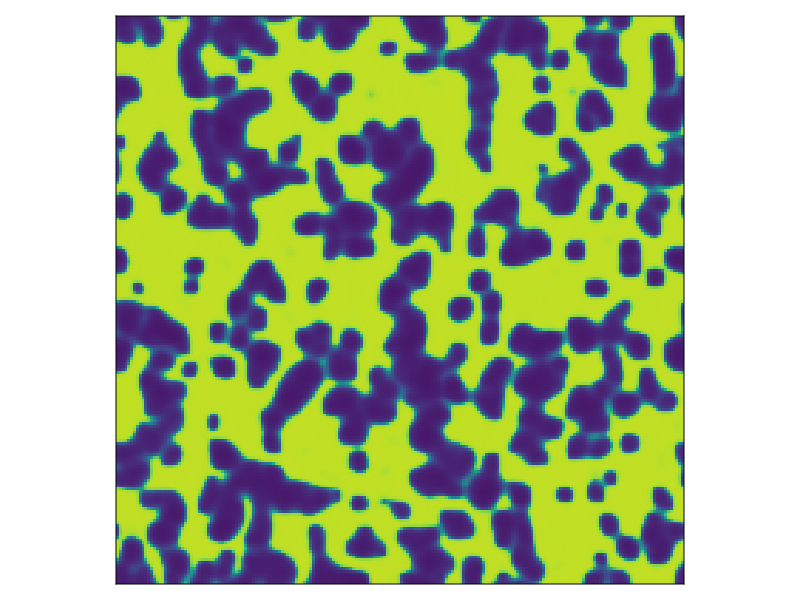
\includegraphics[keepaspectratio, width = \linewidth]{../figures/fig3.9.2.6.png}
    \end{subfigure}
    \hfill
    \begin{subfigure}[b]{0.11\textwidth}
        \centering 
        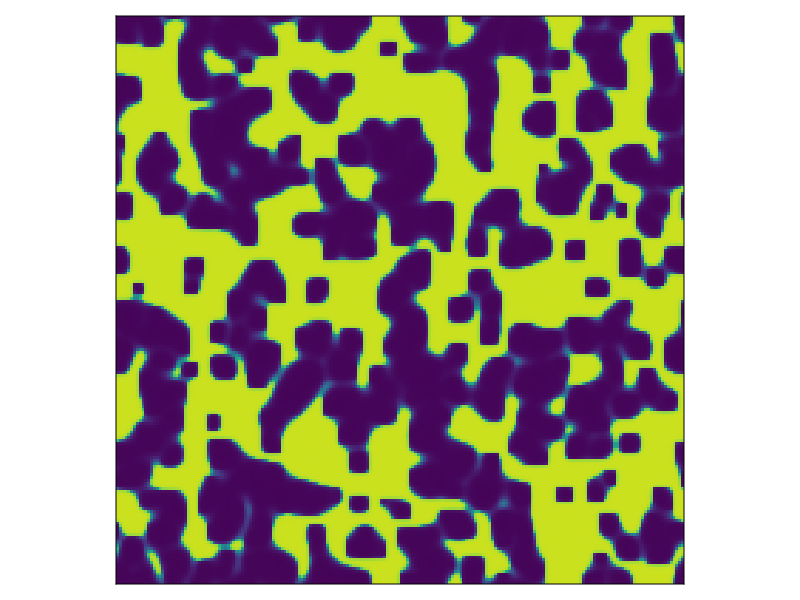
\includegraphics[keepaspectratio, width = \linewidth]{../figures/fig3.9.2.7.png}
    \end{subfigure}
    \hfill
    \begin{subfigure}[b]{0.11\textwidth}
        \centering 
        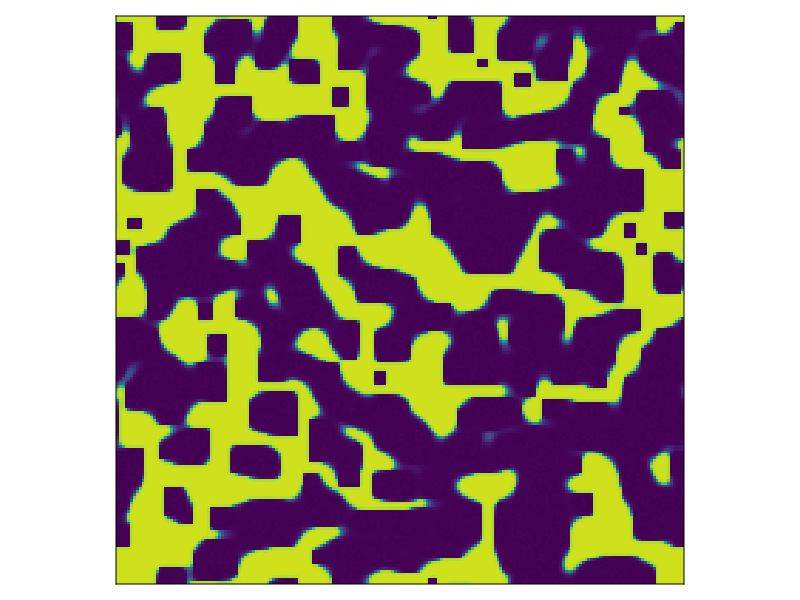
\includegraphics[keepaspectratio, width = \linewidth]{../figures/fig3.9.2.8.png}
    \end{subfigure}
    \caption{Time evolution of the lung ventilation LDS on a square $300\times300$ lattice with slow ($\varepsilon=10^{-2}$), linear ramping of the parameter and noise level $\sigma=10^{-3}$. 
    In the top panel the leading mode of the DMD is reported, showing an abrupt upward burst shortly before the formation of patterns (dashed vertical line). 
In the bottom pannel several snapshots increasing timesteps are reported.}
    \label{fig3.9}
\end{figure}
\end{document}
